\section{Purity Measurement}
\label{sec:purity}
While the isolation requirements described in Section~\ref{sec:isolation} remove the bulk of the neutral-meson background, a substantial contribution remains; in particular, multi-jet events that produce a $\pi^{0}$ or $\eta$ that carries most of the jet energy can pass the selection. Given that the cross-section to produce a $\pi^{0}$ is much larger than the cross-section for prompt photons~\cite{Arleo:2004gn}, the background is still large for the $\pt$ range that we are interested in. In this section, we show measurements of the purity of our $\gammaiso$-candidate sample done with a template-fit method.

\subsection{Template fit method}
The purity of the isolated photon sample is determined with a two-component template fit, as was done for example by the CMS collaboration in Ref.~\cite{Sirunyan:2017qhf}. The distribution of the shower shape variable for the isolated cluster sample is fit to a linear combination of the signal distribution and the background distribution. The shape of the signal distribution is determined by a photon-jet simulation (see Table~\ref{tab:MCsamples}) and the shape of the background distribution is determined from data using an anti-isolated sideband~\footnote{The inversion of an isolation cut to estimate QCD background is a standard technique in several measurements and searches at the LHC and previous hadron colliders.} with an additional correction computed from a dijet simulation. This is described in more detail in the following sections.  

\subsubsection{Signal template and background templates }
We estimate the shape of the background distribution of the shower-shape for isolated clusters with a sideband technique. That is, we estimate the shower shape distribution of clusters from isolated decay photons with clusters that are anti-isolated but pass all other selection criteria. This method assumes that the correlation between the isolation variable and shower shape variable can be corrected for; the procedure for doing so is described below. The signal and sideband regions defined using the isolation variable are illustrated in Figure~\ref{SidebandDefinition}. 

\begin{figure}[h]
\center
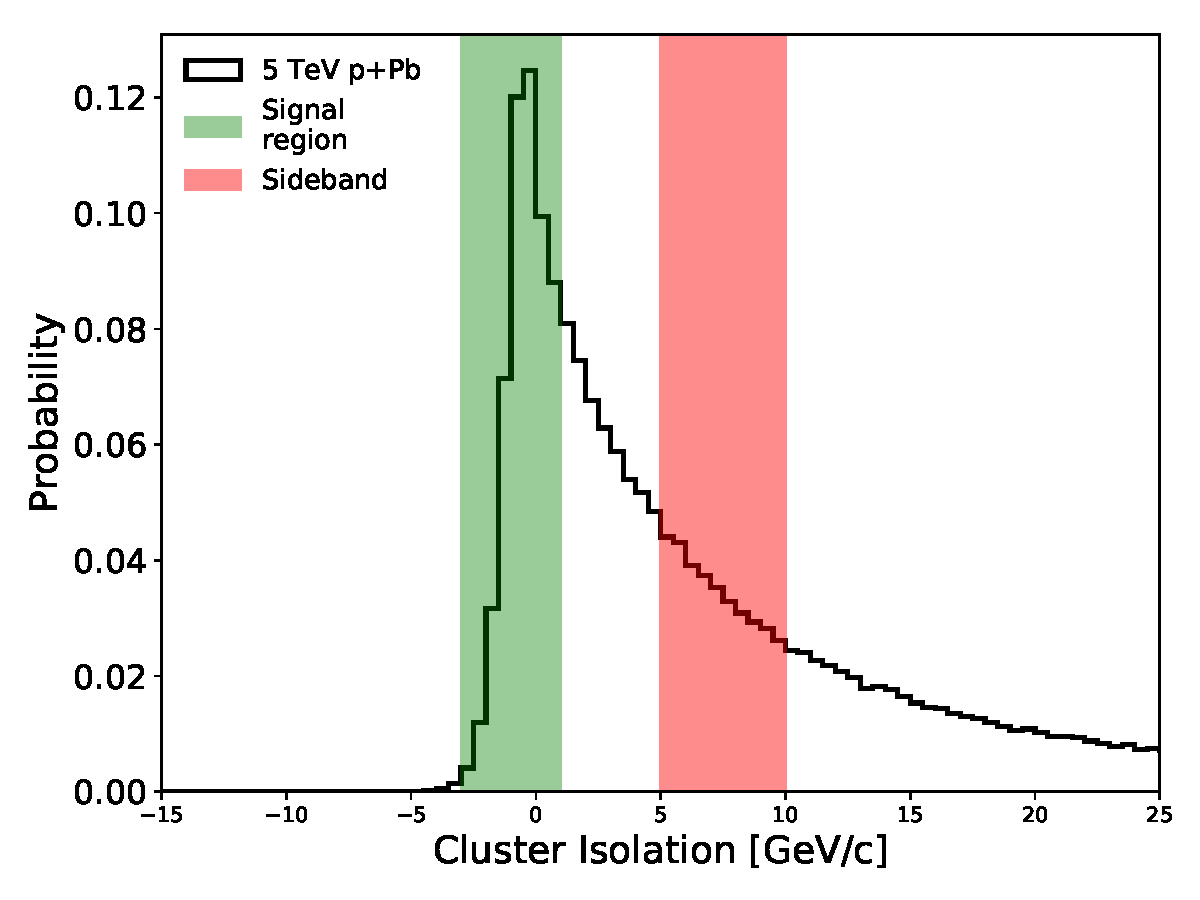
\includegraphics[width=0.49\textwidth]{Purity/IsolationSideband_limited_Skimmed_13def_root}
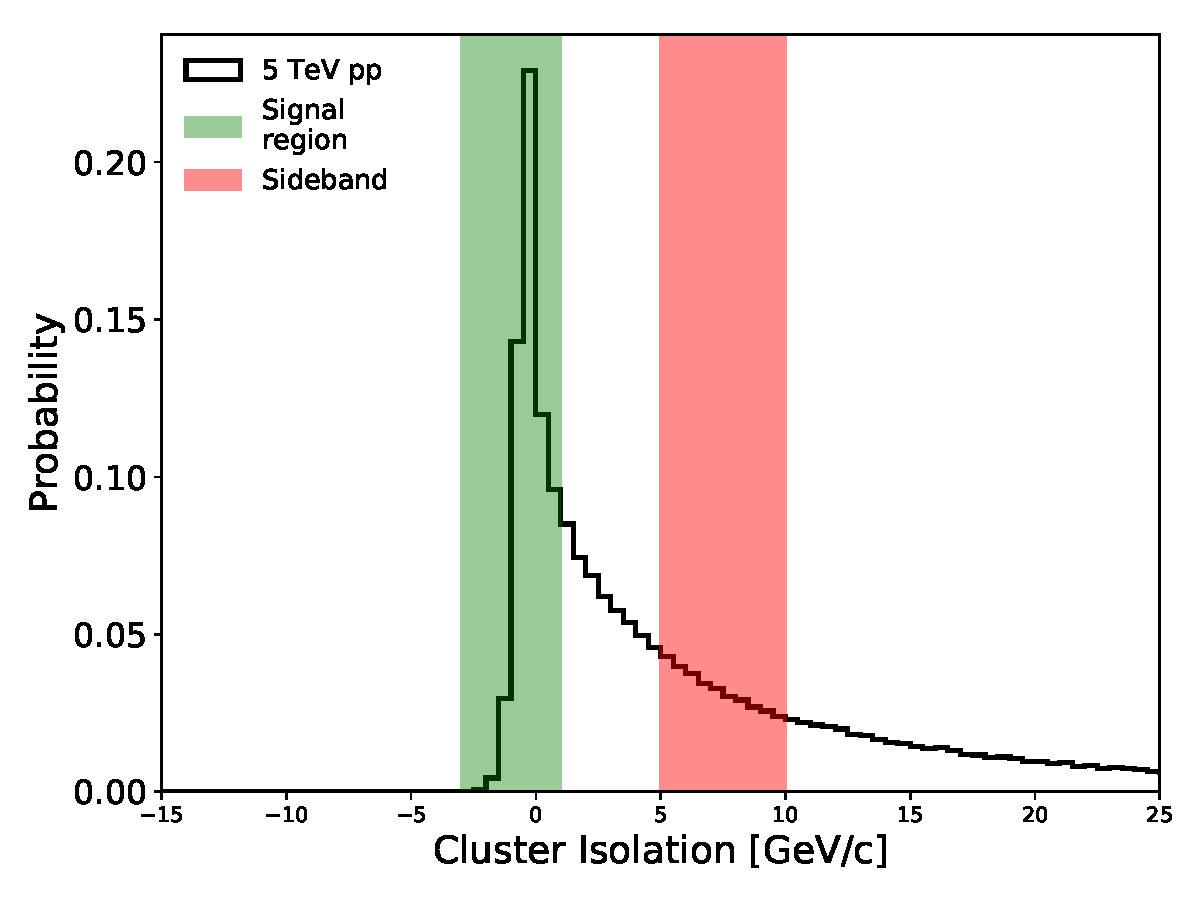
\includegraphics[width=0.49\textwidth]{Purity/IsolationSideband_limited_Skimmed_17q_root}
\caption{Isolation variable distribution of clusters with $\pt$ between 12 and 16 \GeVc~in \pPb~data (left panel) and pp data (right panel). The green shaded are represents the signal region ($\iso<$ 1.5 \GeVc); the red represent the sideband ($5<\iso<10$ \GeVc) used to estimate the background template.}
\label{SidebandDefinition}
\end{figure}

For simplicity, the same definitions are used for pp and \pPb~data. The lower bound of the sideband region is defined as {$\iso=5$ \GeVc}; according to photon-jet simulations, less than 1$\%$ of prompt photons are beyond this range. The upper bound is chosen such that the sideband is as narrow as possible, to minimize a possible bias to the shower-shape distribution due to a positive correlation with ISO, while still containing a number of clusters comparable to the signal region. A more rigorous study on the sensitivity of our purity estimate on the choice of sideband region is shown in Section~\ref{sec:bkgtemplate}.

Figure~\ref{TemplateShapes} summarizes the signal and background templates used in the template fit. The distributions are rather different, which is key for the stability of the template fit. The background shape in the $\lambdasquare$ variable shows a peak in the single-shower region but a ``bump'' that reflects a $\pi^{0}$ peak. In both cases, the peaks in the single-shower region that are observed in the background templates come mostly from collinear $\pi^{0}\to\gamma\gamma$ decays.

\begin{figure}
\center
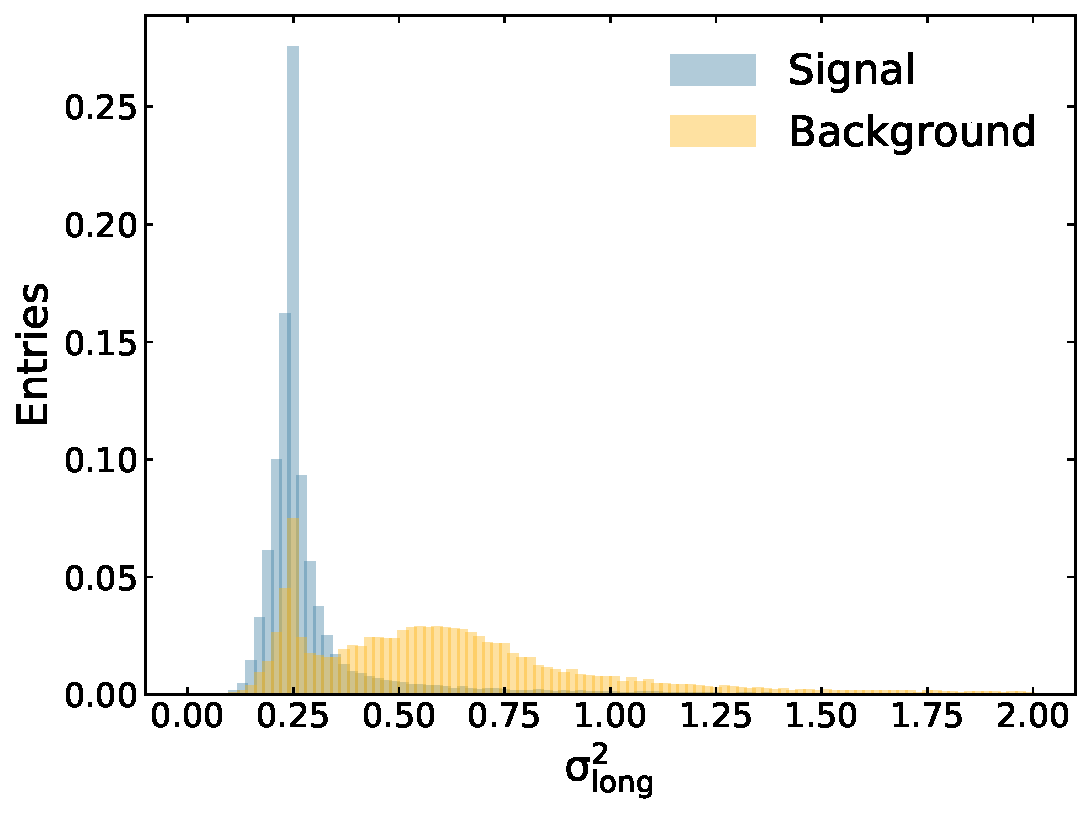
\includegraphics[width=0.49\textwidth]{Purity/norm-templates-p-Pb-cluster_Lambda-15-20.pdf}
\caption{Normalized signal (blue) and background (yellow) distributions used as input for the template fit. These distributions correspond to clusters with \pt~in the 15--20 \GeVc~range.}
\label{TemplateShapes}
\end{figure}

The background template is corrected for the correlation between the shower shape distribution and the isolation energy. A dijet simulation is used to construct the ratio of the shower shape distribution for isolated clusters to the shower shape distribution for anti-isolated clusters. This ratio, as a function of shower shape variable, is then applied as a weight to the anti-isolated clusters in the data, giving a corrected background template that is then used in the template fit (see Equation~\ref{eq:bkgtemplatecorrection}). From this equation, it is clear that, if the MC exactly replicates the data, the Weights function exactly corrects the anti-isolated decay photon \lambdasquare distribution back to the isolated decay photon \lambdasquare~distribution, which is the true background. 

\begin{align}
    \text{Weights}(\lambdasquare)&=\frac{\text{Iso}_{\text{MC}}(\lambdasquare)}{\text{Anti-iso}_{\text{MC}}(\lambdasquare)} \nonumber \\
    \text{Bkg}^{\text{corrected}}(\lambdasquare)&=\text{Non-iso}_{\text{data}}(\lambdasquare)\times\text{Weights}(\lambdasquare)
    \label{eq:bkgtemplatecorrection}
\end{align}

The purity as computed with the corrected background template is 8--13\% lower in absolute value as compared to the purity as computed with the uncorrected background template; an example of a fit with and without the correction is shown in Figure~\ref{fig:purcorrectionexample}. The correction greatly improves the goodness-of-fit. The $\text{Weights}(\lambdasquare)$ function for different \pt~ranges is shown in Appendix~\ref{sec:MCbasedcorrection} and the evaluation of the systematic uncertainty associated with this correction is described in Section~\ref{sec:puritysystematics}. 

\FloatBarrier
\begin{figure}
    \centering
    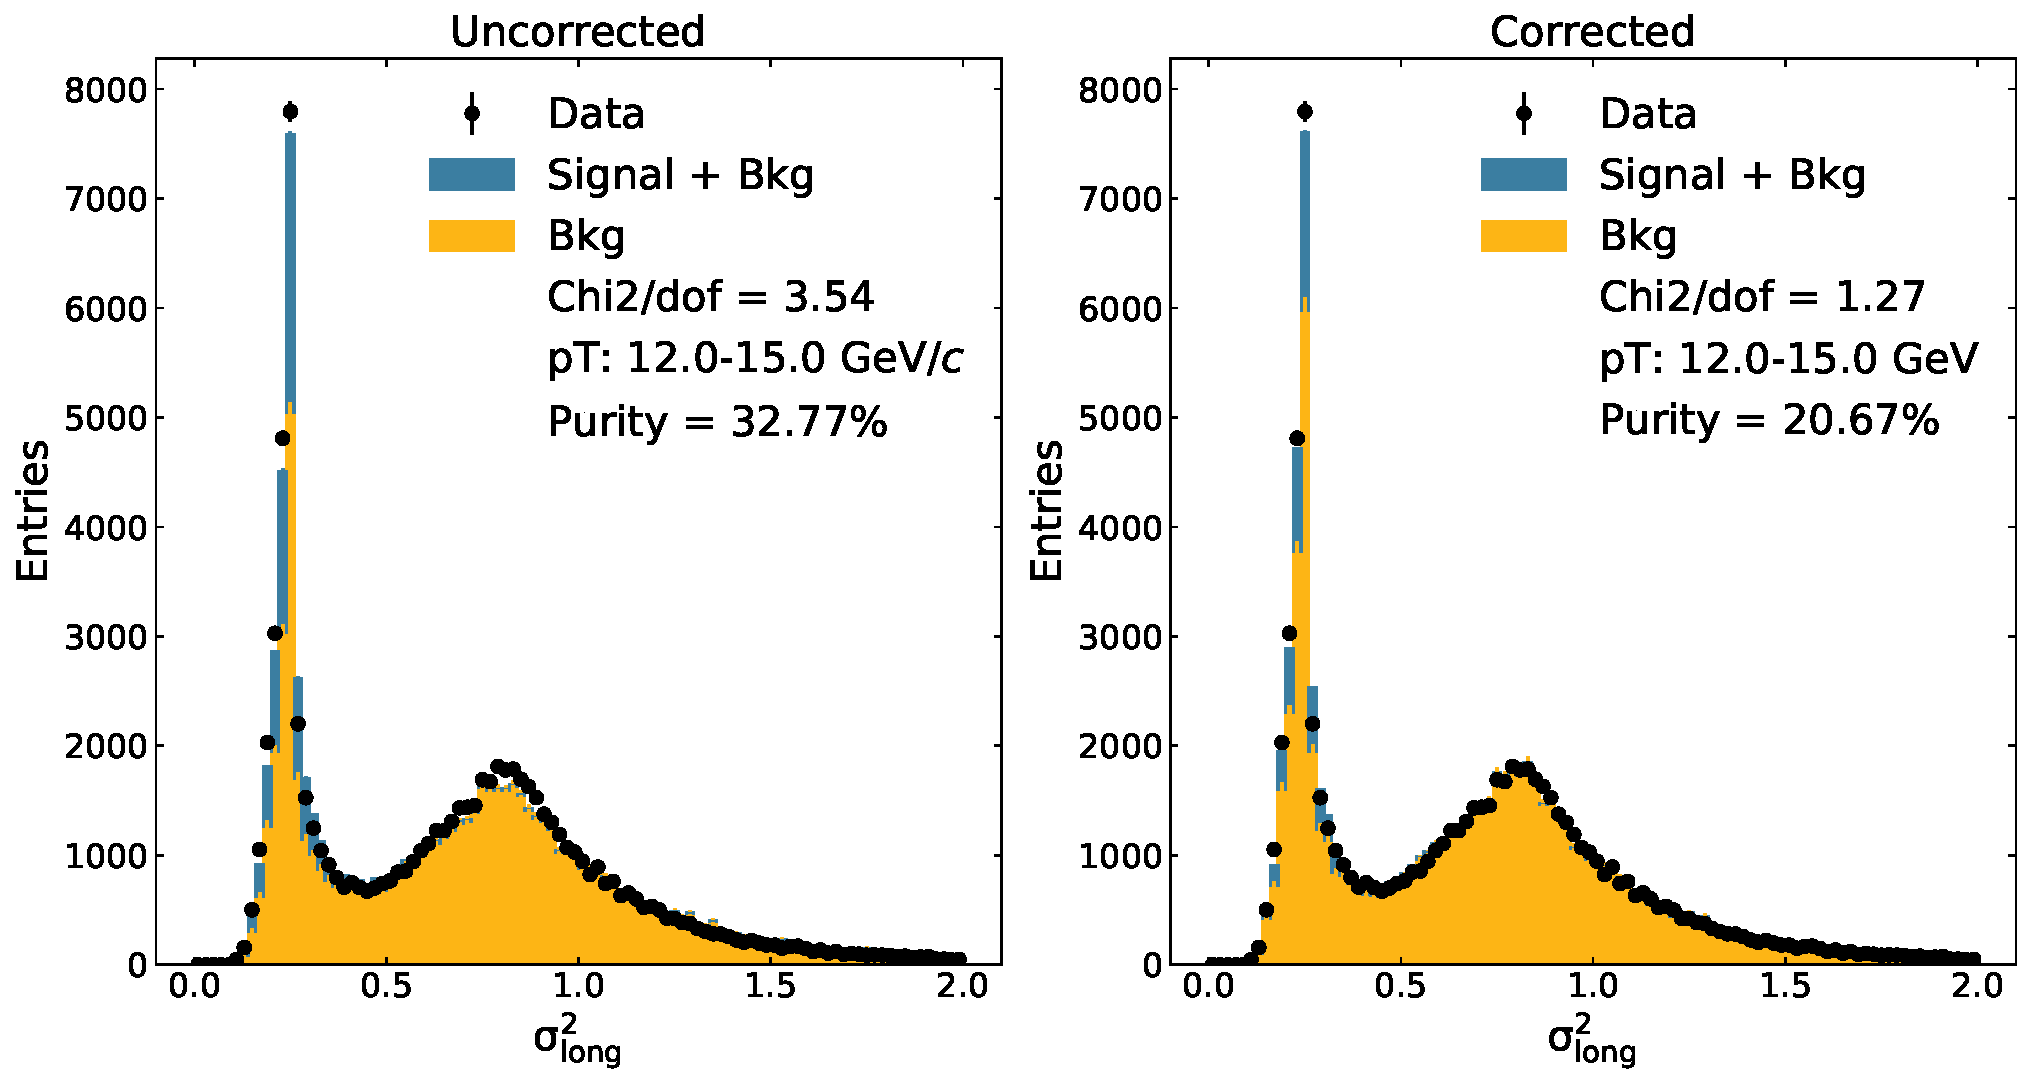
\includegraphics[width=\textwidth]{Purity/correction-example-p-Pb-cluster_Lambda-12-15.pdf}
    \caption{An example of the template fit with and without the background template correction in \pPb~for clusters with $12 < \pt < 15$ GeV/$c$. The goodness of fit is better after the correction and the purity is significantly lower.}
    \label{fig:purcorrectionexample}
\end{figure}


\subsubsection{Fit results}
\label{sec:fitresults}
The distribution of isolated clusters is fit with a linear combination of the signal and background templates. We use the \textsc{MINUIT}~\cite{James:1975dr} package for $\chi^{2}$ minimization and the \textsc{MIGRAD} package for error estimation. The only free parameter in the fit is the number of signal clusters, $N_{\mathrm{sig}}$, because the overall normalization, $N$, is fixed to the total number of isolated clusters:
\begin{equation}
N^{\mathrm{observed}} = N_{\mathrm{sig}}\times S + (N-N_{\mathrm{sig}})\times B,
\end{equation}
where $S$ and $B$ are the normalized signal template and background template. 


Figures~\ref{TemplatefitResults_Preliminary} show template fit results for \pPb~and pp data. In all cases a good fit with no systematic pattern in the residuals is achieved over most of the distribution, and the reduced $\chi^{2}$ ranges within acceptable values. The purity measurements are presented in graphical form in Figure~\ref{fig:purityresults}. 


\begin{figure}[h]
\center
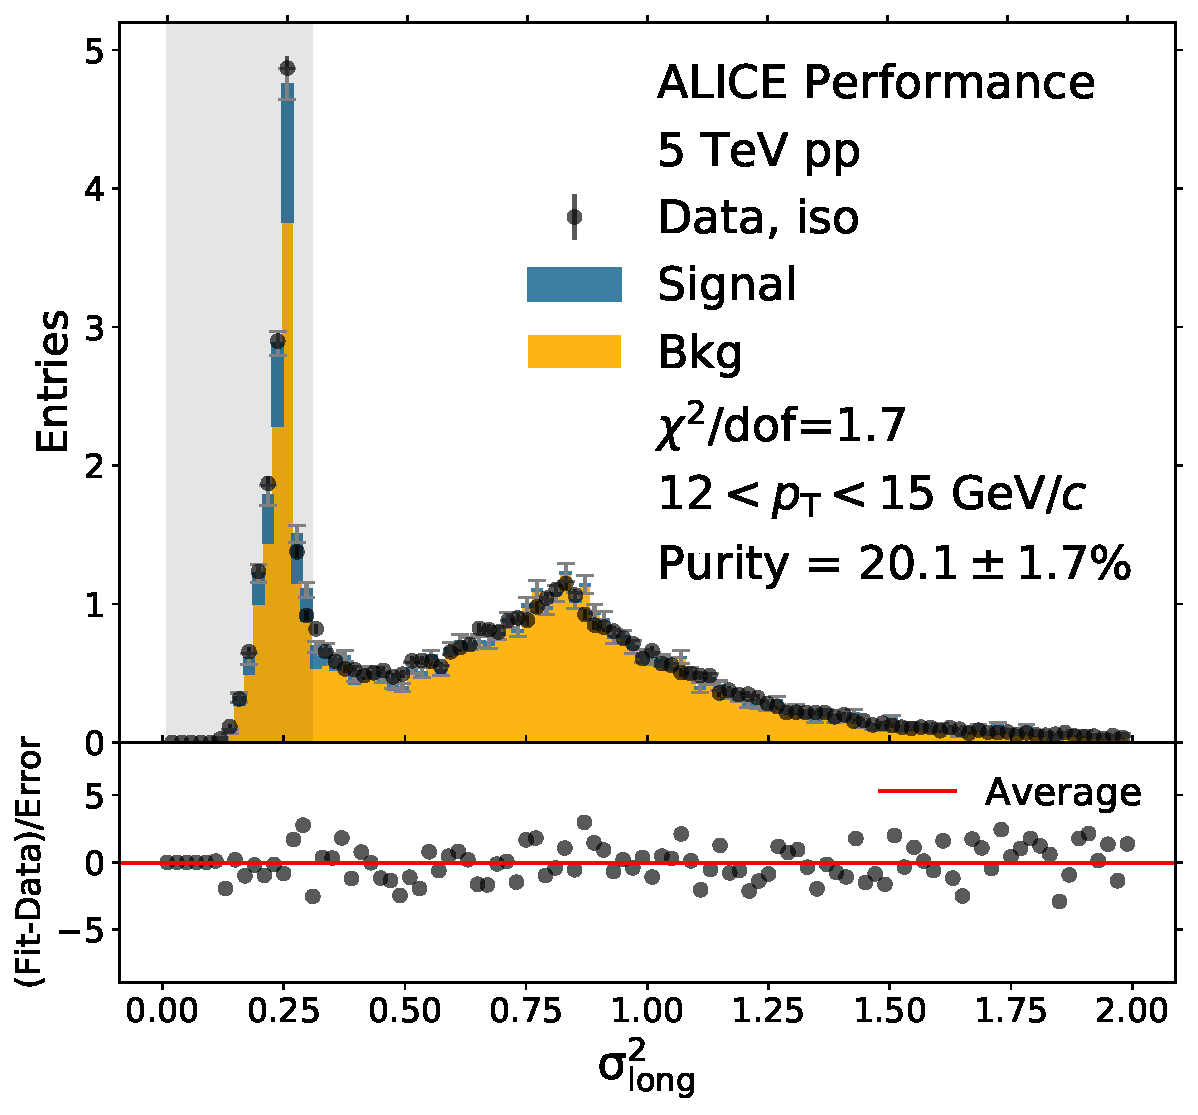
\includegraphics[width=0.38\textwidth]{Purity/tf-example-pp-cluster_Lambda-12-15.pdf}
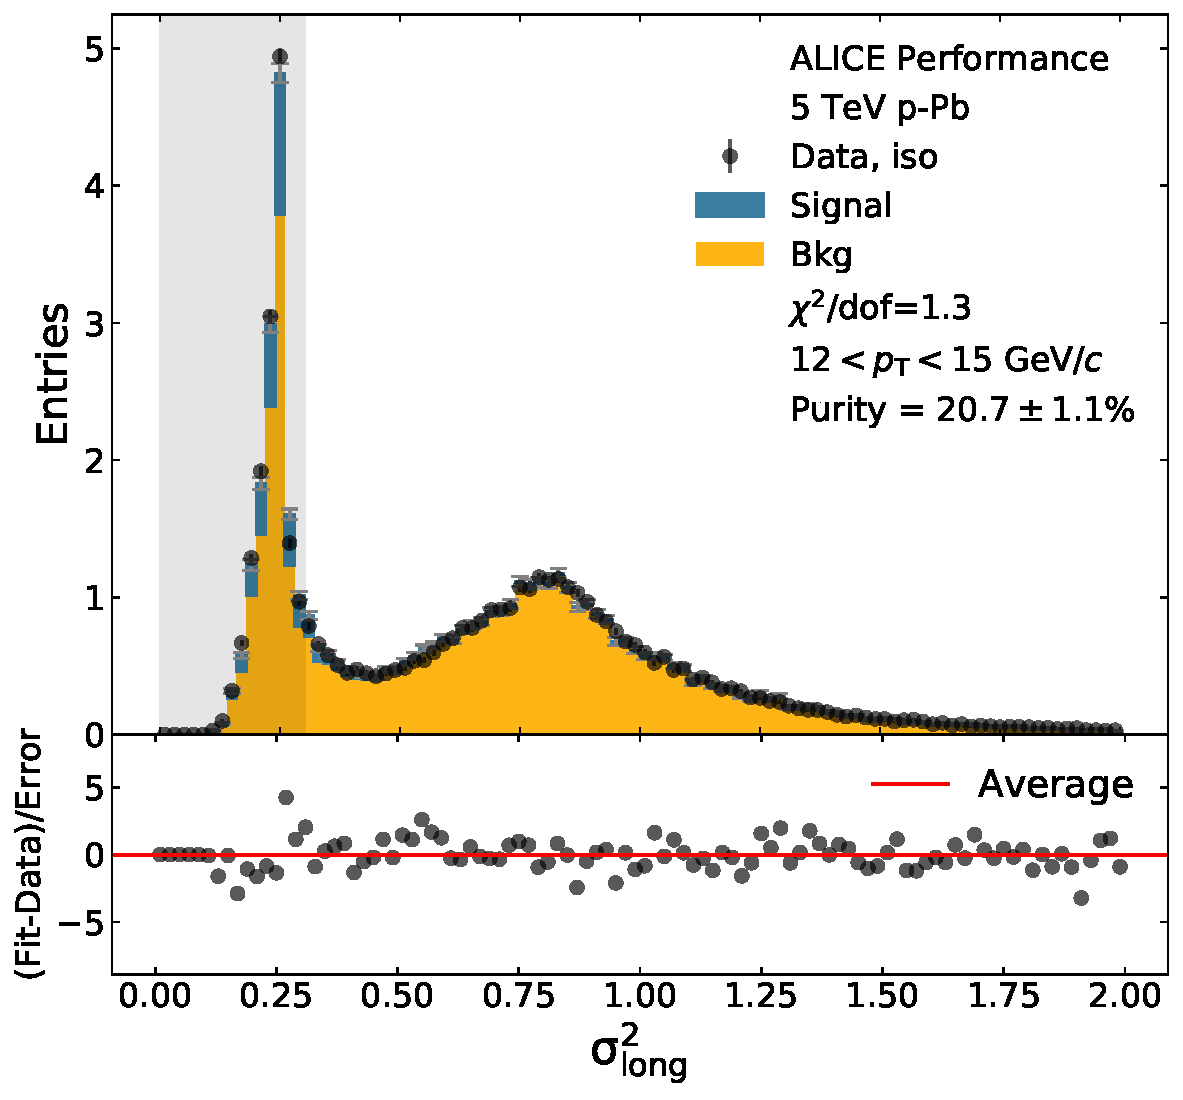
\includegraphics[width=0.38\textwidth]{Purity/tf-example-p-Pb-cluster_Lambda-12-15.pdf}
\\
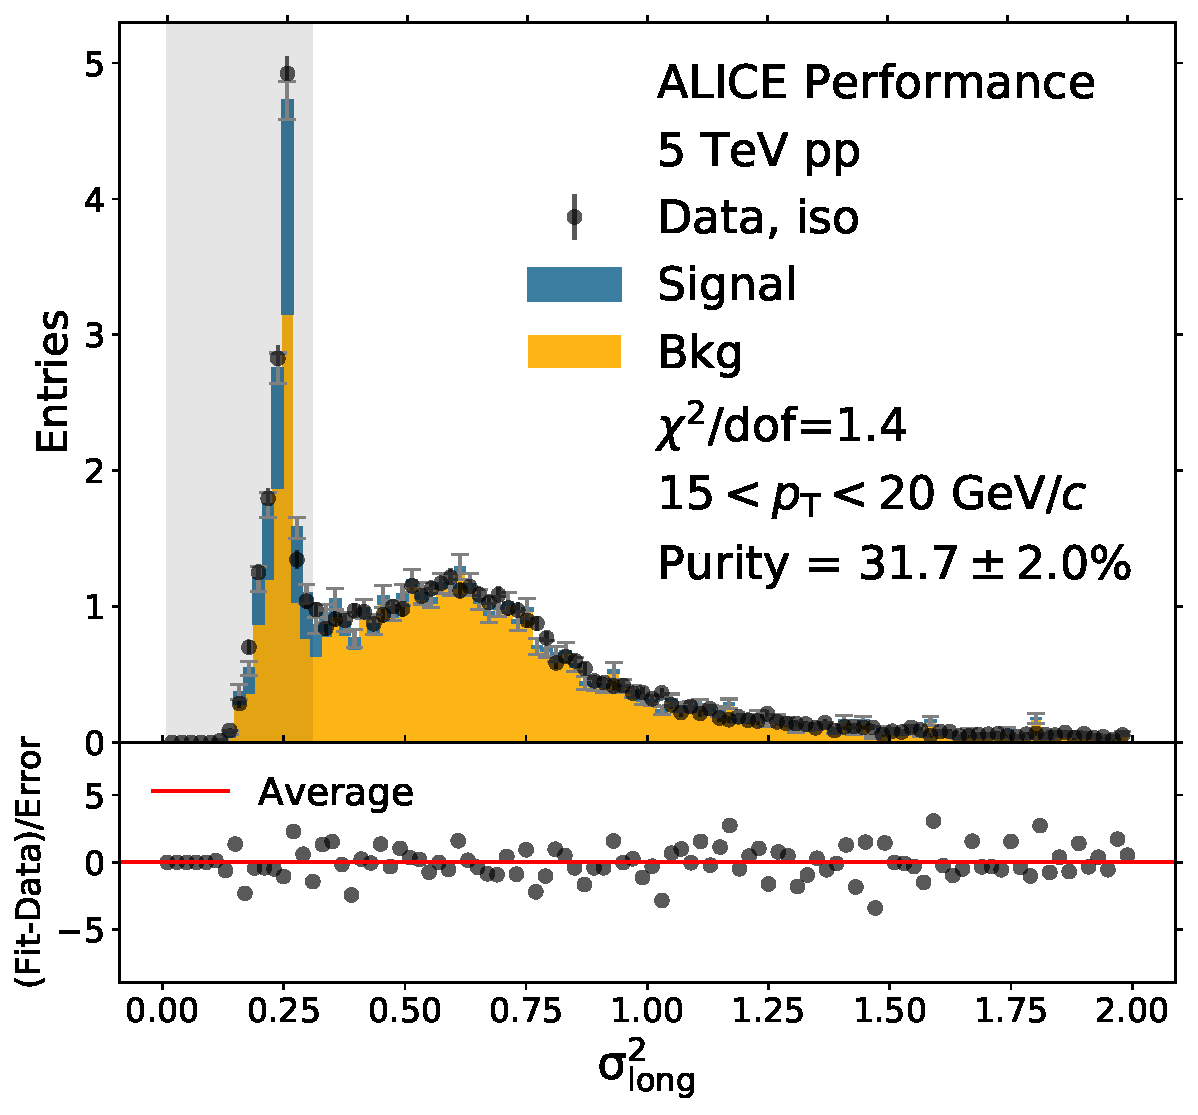
\includegraphics[width=0.38\textwidth]{Purity/tf-example-pp-cluster_Lambda-15-20.pdf}
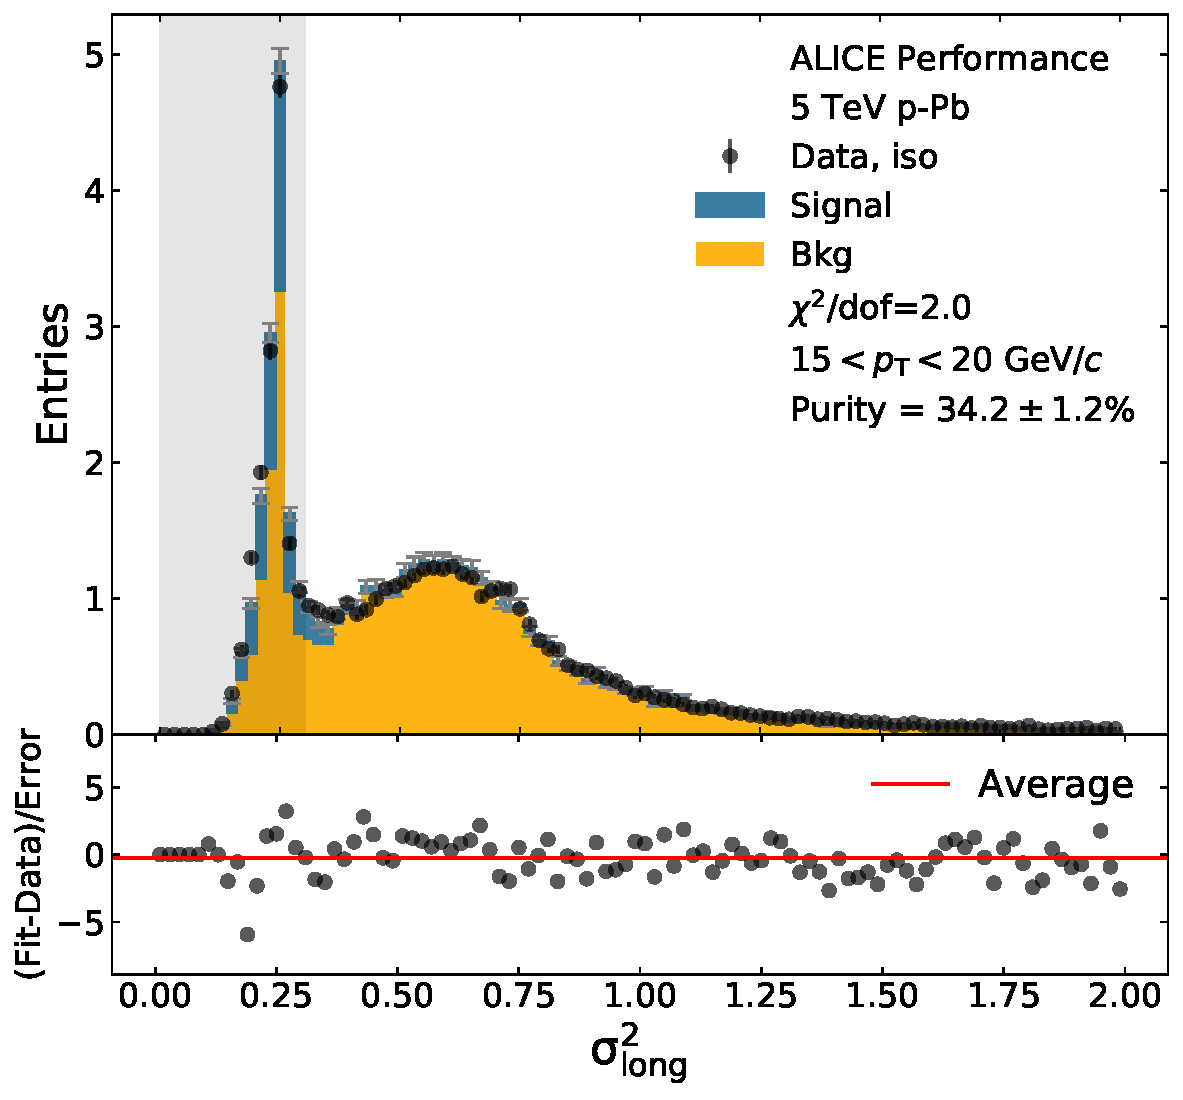
\includegraphics[width=0.38\textwidth]{Purity/tf-example-p-Pb-cluster_Lambda-15-20.pdf}
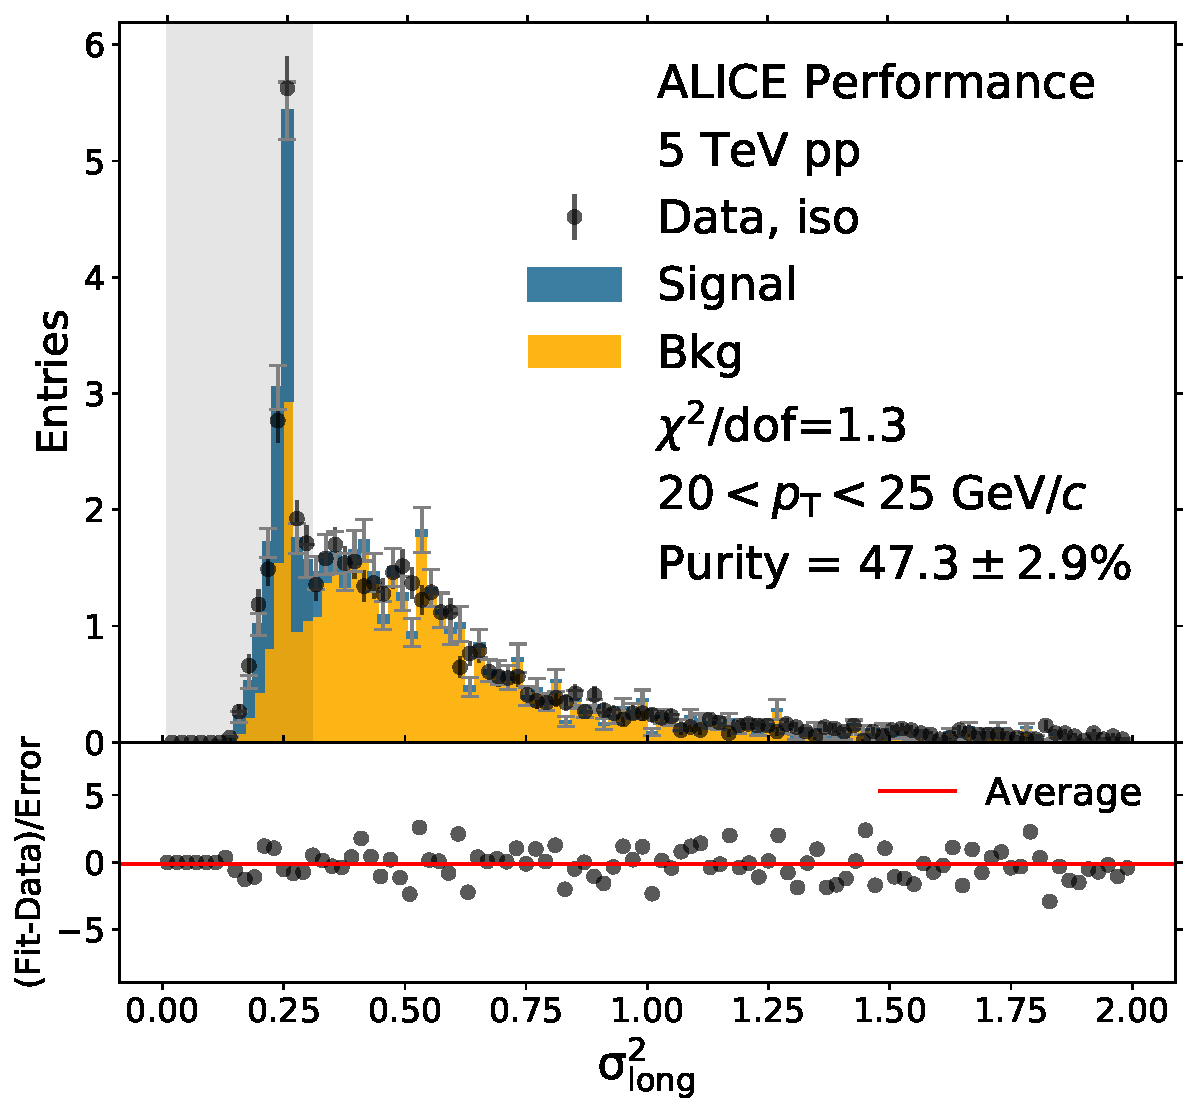
\includegraphics[width=0.38\textwidth]{Purity/tf-example-pp-cluster_Lambda-20-25.pdf}
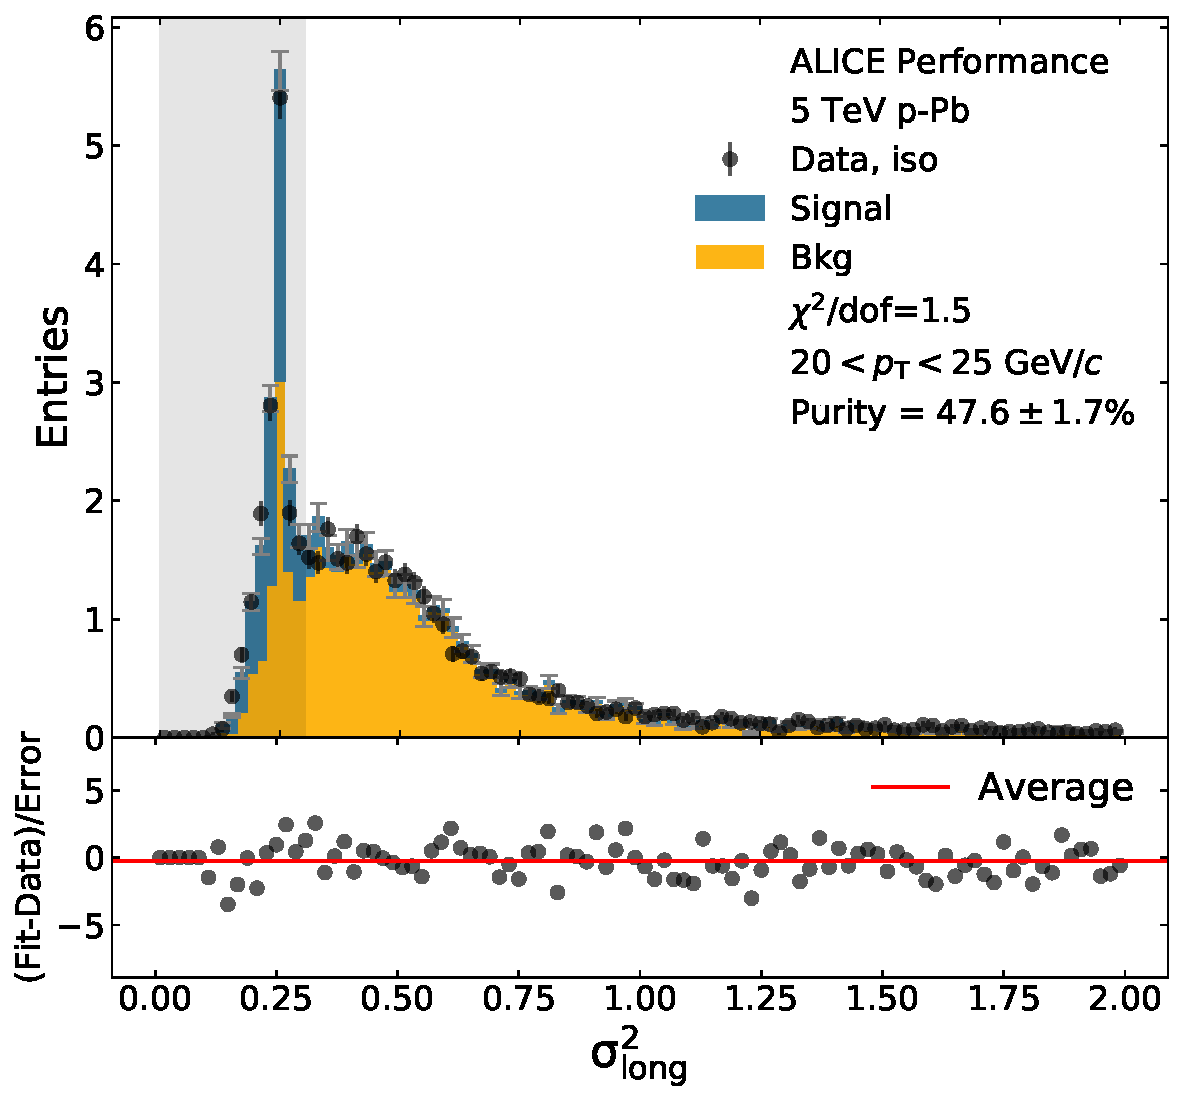
\includegraphics[width=0.38\textwidth]{Purity/tf-example-p-Pb-cluster_Lambda-20-25.pdf}
\\
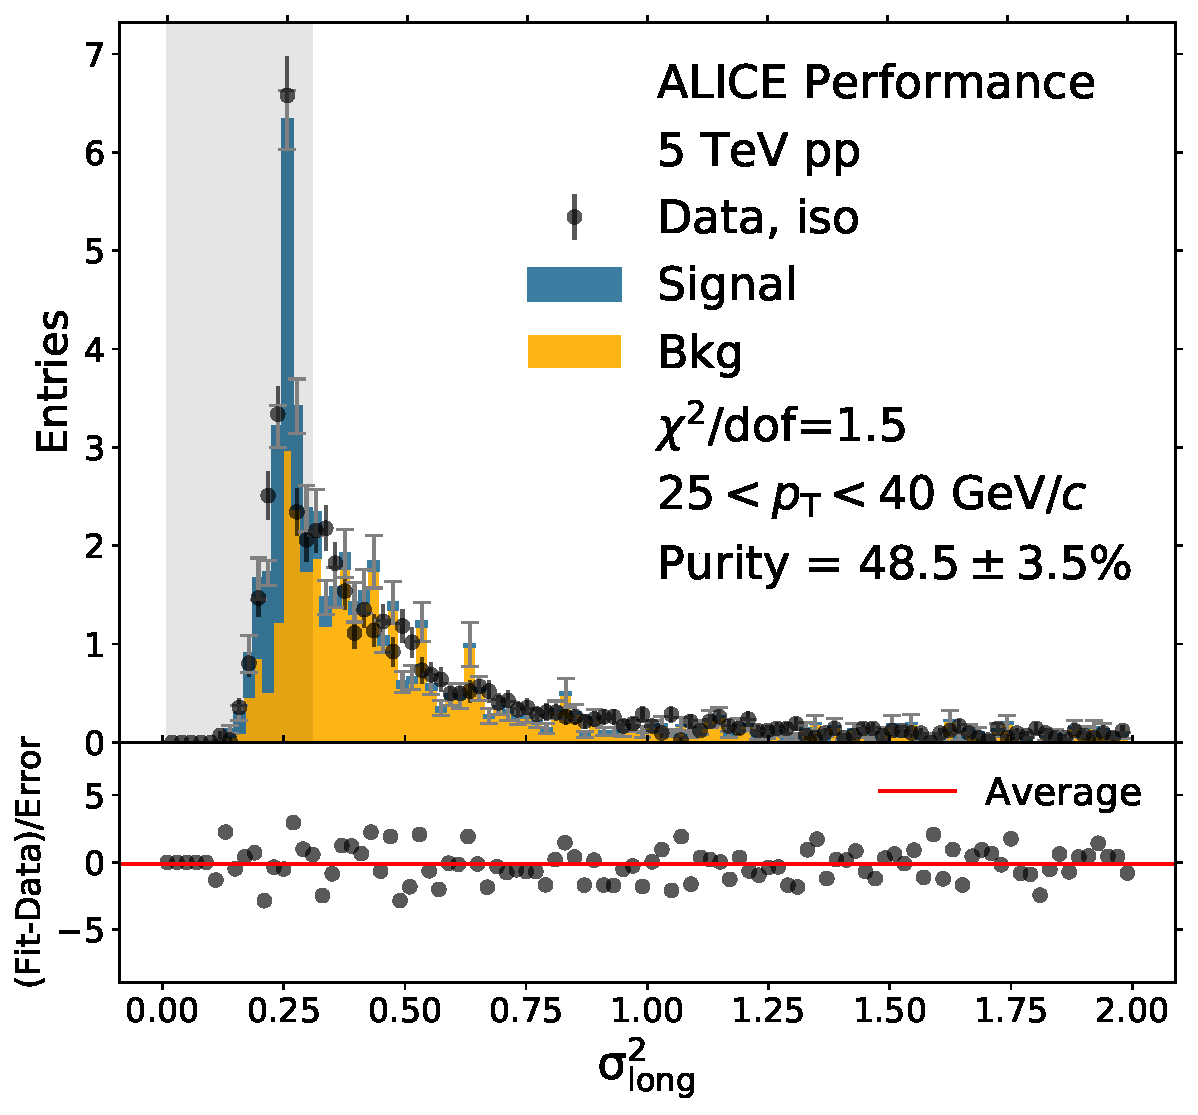
\includegraphics[width=0.38\textwidth]{Purity/tf-example-pp-cluster_Lambda-25-40.pdf}
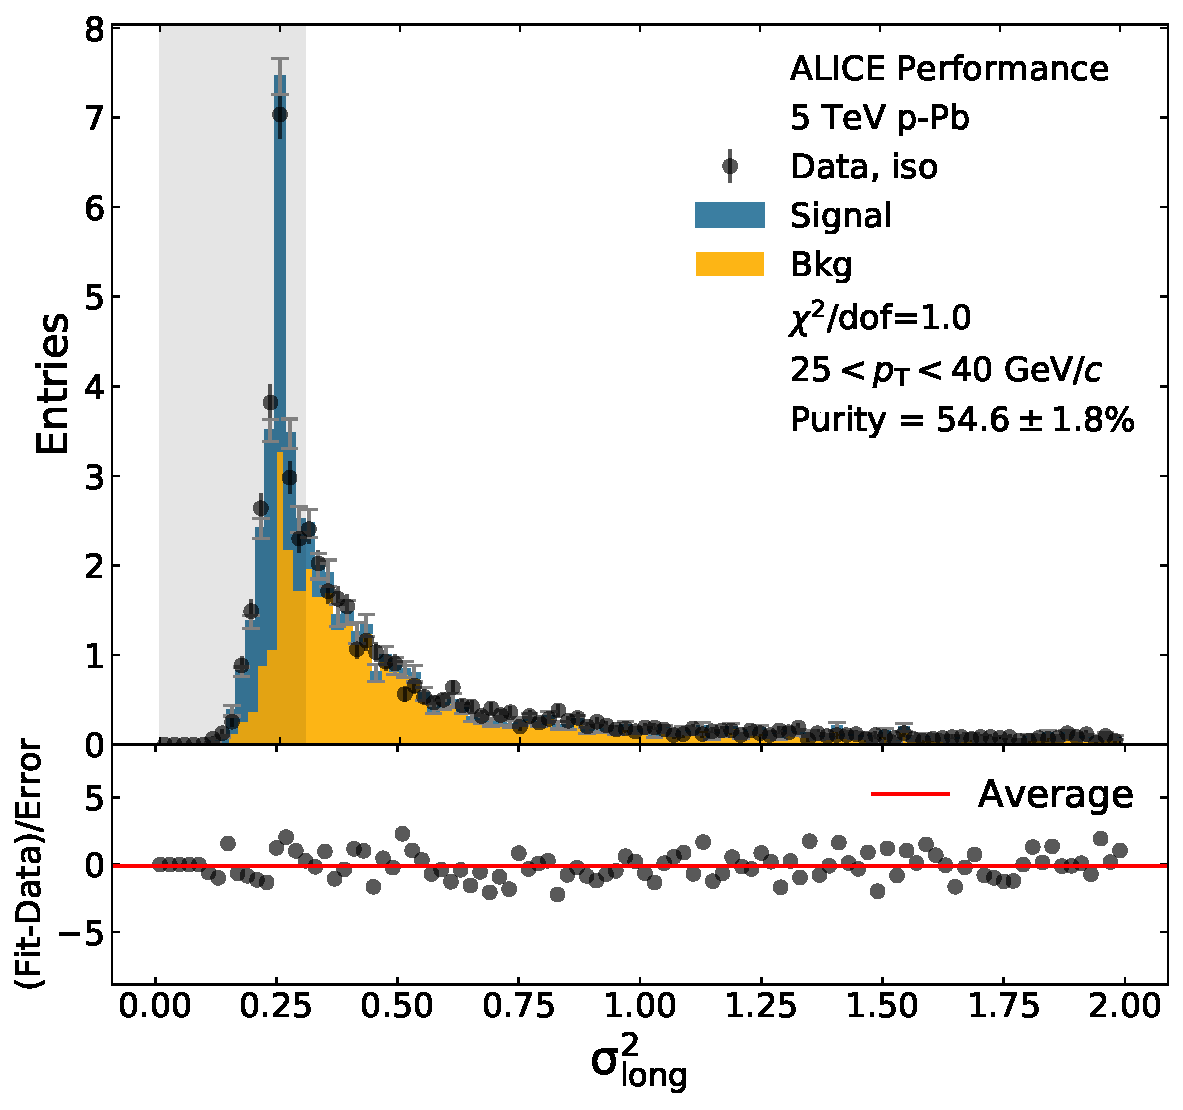
\includegraphics[width=0.38\textwidth]{Purity/tf-example-p-Pb-cluster_Lambda-25-40.pdf}
\caption{Template fit results in pp and \pPb~data. The stacked histograms (yellow for background, blue for signal) are the predicted counts given the best-fit value of the number of signal photons, $N_{\mathrm{sig}}$. The hatched gray area represents the interval considered for the purity estimate. The bottom panels show the normalized residuals of the fit, considering the statistical uncertainty on the isolated cluster data and the background template added in quadrature. }
\label{TemplatefitResults_Preliminary}
\end{figure}

%\begin{table}
%   \caption{Impact of the \gammaiso selection variations on purity measurement on pp and \pPb~data. The nominal isolation selection is changed to $\iso<$1.50 $\pm$ 0.25 \GeVc; the nominal shower-shape selection is changed to  $\lambdasquare<0.30 \pm 0.03$}
%   \label{tab:variationspurity}
    % \begin{tabular*}{1.0\columnwidth}{@{\extracolsep{\fill}}l|llllll@{}}
    % 	\hline
    % 	 & Nominal & $\iso < 1.25$ \GeVc & $\iso < 1.75$ \GeVc & $\lambdasquare < 0.27$ & $\lambdasquare < 0.33$ \\
    % 	\hline
    % 	pp data & & & & & \\
    % 	\hline
    % 	12--15 \GeVc & 16.9 & 18.2 & 15.9 & 16.5 & 16.9 \\
    % 	15--20 \GeVc & 29.5 & 31.0 & 28.0 & 29.3 & 29.1 \\
    % 	20--25 \GeVc & 46.8 & 48.4 & 45.4 & 49.1 & 44.9 \\
    % 	25--40 \GeVc & 48.0 & 49.3 & 46.7 & 55.9 & 45.1 \\
    % 	\hline
    % 	p-Pb data & & & & & \\
    % 	\hline
    % 	12--15 \GeVc & 20.7 & 21.5 & 19.7 & 20.2 & 20.5 \\
    % 	15--20 \GeVc & 34.2 & 35.5 & 33.1 & 34.3 & 33.6 \\
    % 	20--25 \GeVc & 47.6 & 49.0 & 46.5 & 51.7 & 44.9 \\
    % 	25--40 \GeVc & 54.6 & 56.8 & 52.8 & 62.1 & 51.1 \\
    % 	\hline
    % \end{tabular*}
%\end{table}









\begin{figure}[h]
\center
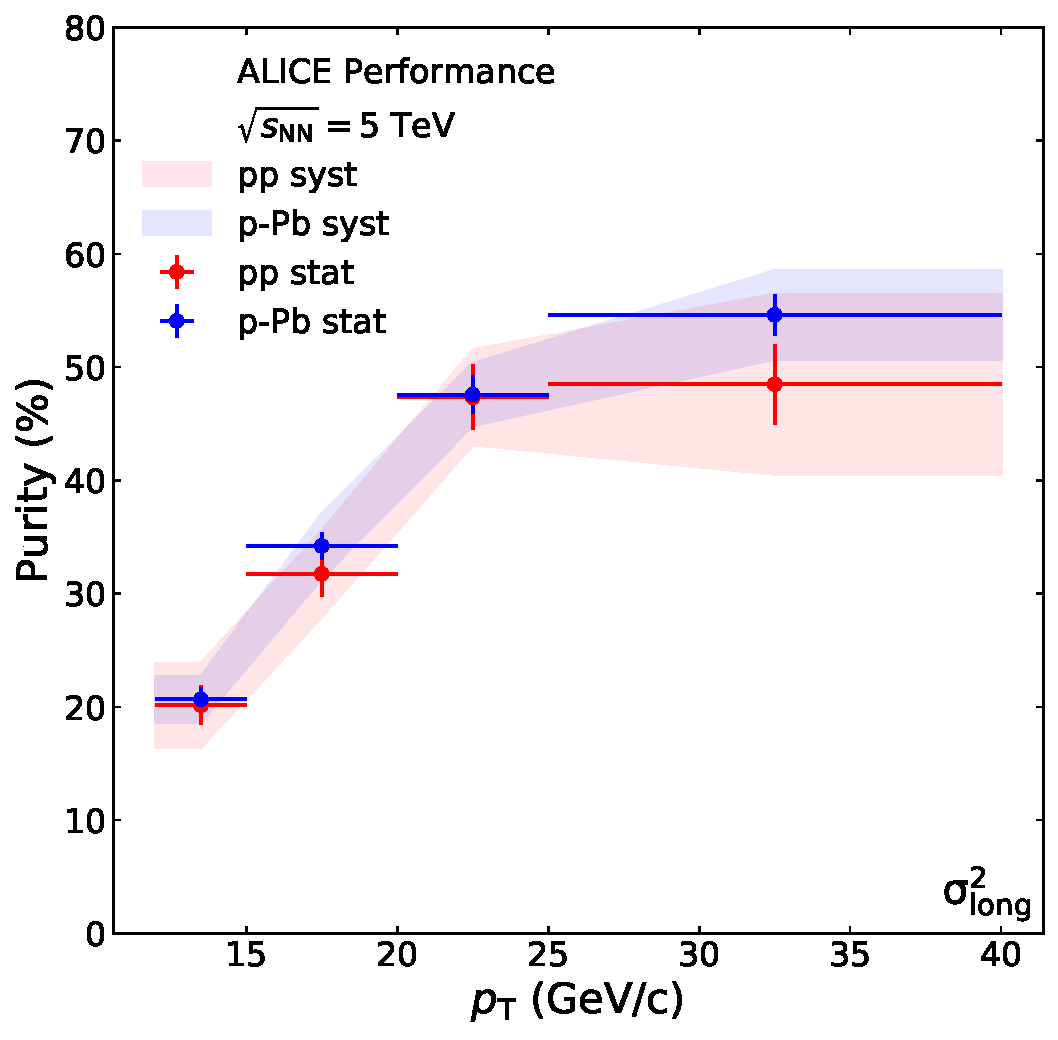
\includegraphics[width=0.495\textwidth]{Purity/purities-combined-cluster_Lambda.pdf}
\caption{Purity of isolated-photon selection as a function of cluster \pt. The error bar represents statistical uncertainty only. The error band represents the systematic uncertainty only.}
\label{fig:purityresults}
\end{figure}

\FloatBarrier
%%%%%%%%%%%%%%%%%%%%%%%%%%%%%%%
\subsection{Systematic uncertainties of the purity measurement}
\label{sec:puritysystematics}
There are two assumptions underlying the template fit procedure. The first is that the signal template from simulations is correct. The second is that the shape of the background estimated from the anti-isolated sideband, with the correction coming from simulations, reflects the shape of the background in the signal region. That is, the assumption is that the correlation between the shower shape and isolation variables can be corrected for via an appropriate simulation. The dominant sources of systematic uncertainty on this measurement are described in this section and can be summarized as follows: the signal template, the sideband region selection, and the background template correction. We also investigated the effect of varying our cluster selection but found that the variations on the purity measurements are much smaller than the other sources of systematic uncertainties investigated here, so we neglect that. This is shown in Appendix~\ref{sec:clustercutselectionvariation}. 

\subsubsection{Signal template}
We estimate the systematic uncertainty on the purity estimate due to imperfections in the signal template by using a data-driven template fit. In this, we restrict the range of the $\chi^{2}$ fit to the background-dominated region of the shower-shape distribution (0.4--1.5 for $\lambdasquare$) and we use only the background template to fit the isolated data with the normalization as the only free parameter. To factorize the effect of the MC-correction to the background template, we do not apply it for this study. Once the background normalization is fitted, we consider the signal to be the integral of the isolated data minus the integral of the background, both in the signal region of the shower-shape variable. 

Figure~\ref{BkgOnlyFit_pPb} show the results obtained with this method in pp and \pPb~data. We observe some systematic pattern in the residuals, which can be attributed to the lack of MC-correction on the background template. 

\begin{figure}[h]
\center
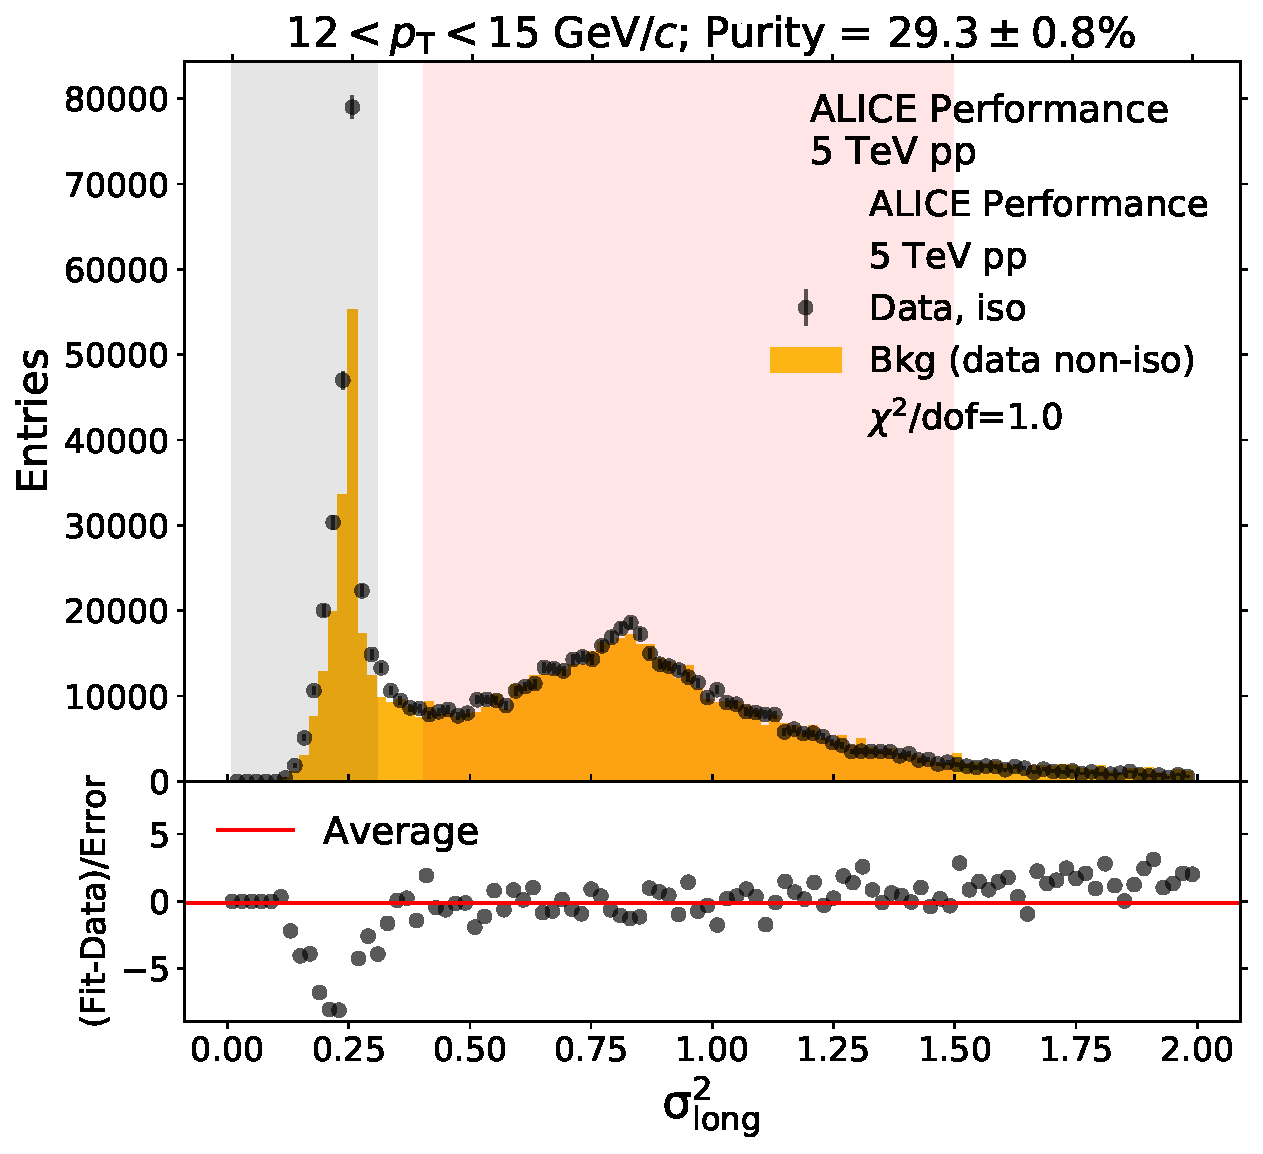
\includegraphics[width=0.38\textwidth]{Purity/bf-example-pp-cluster_Lambda-12-15.pdf}
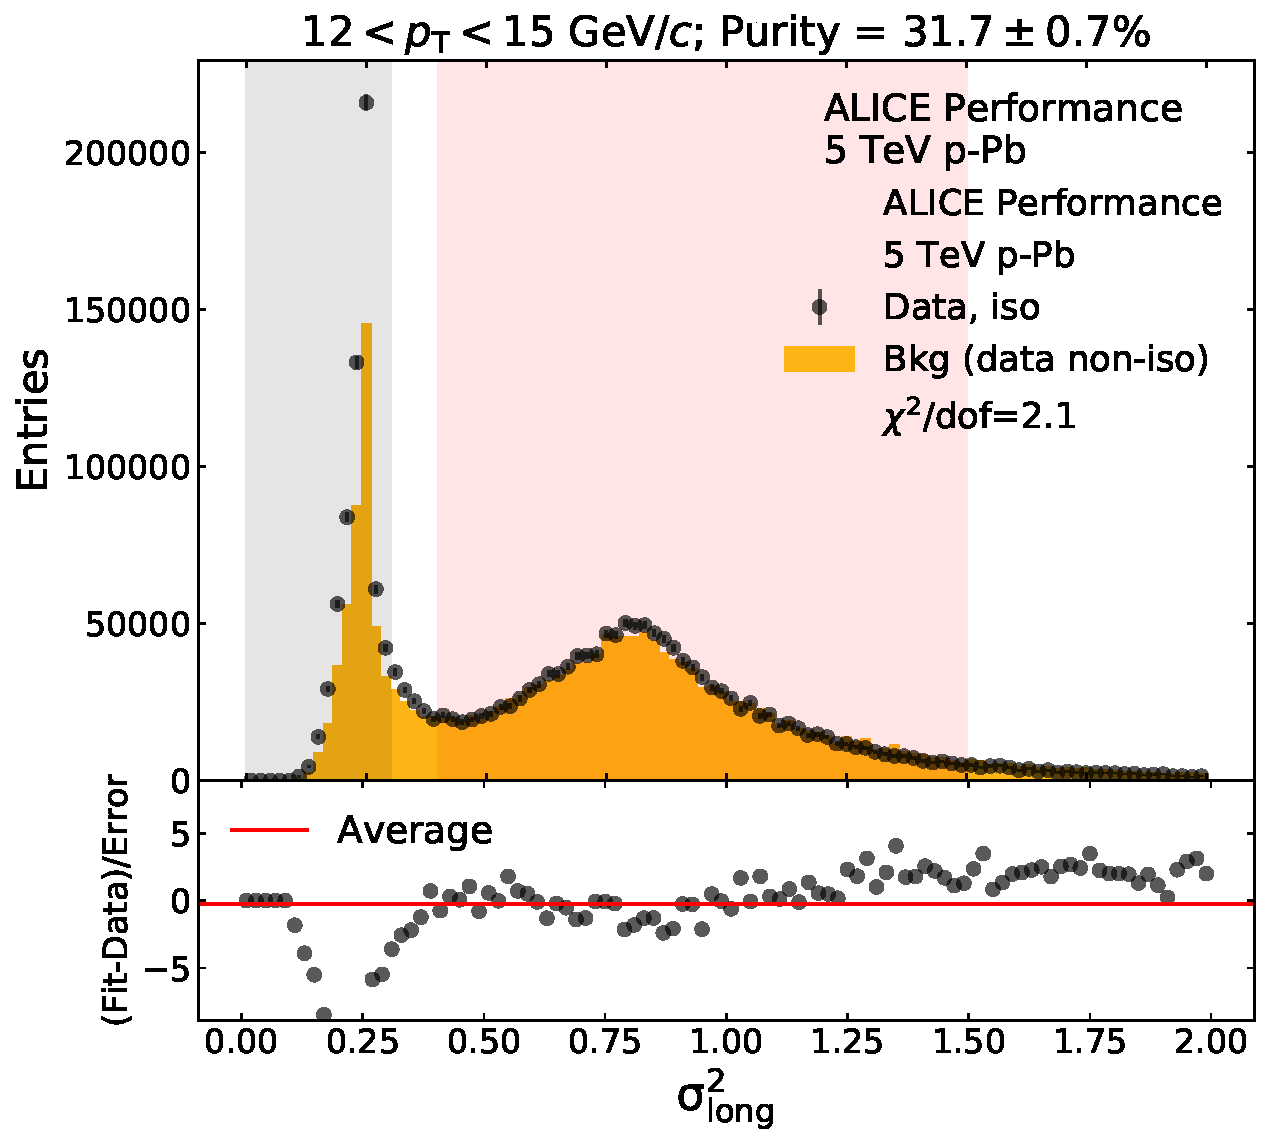
\includegraphics[width=0.38\textwidth]{Purity/bf-example-p-Pb-cluster_Lambda-12-15.pdf}
\\
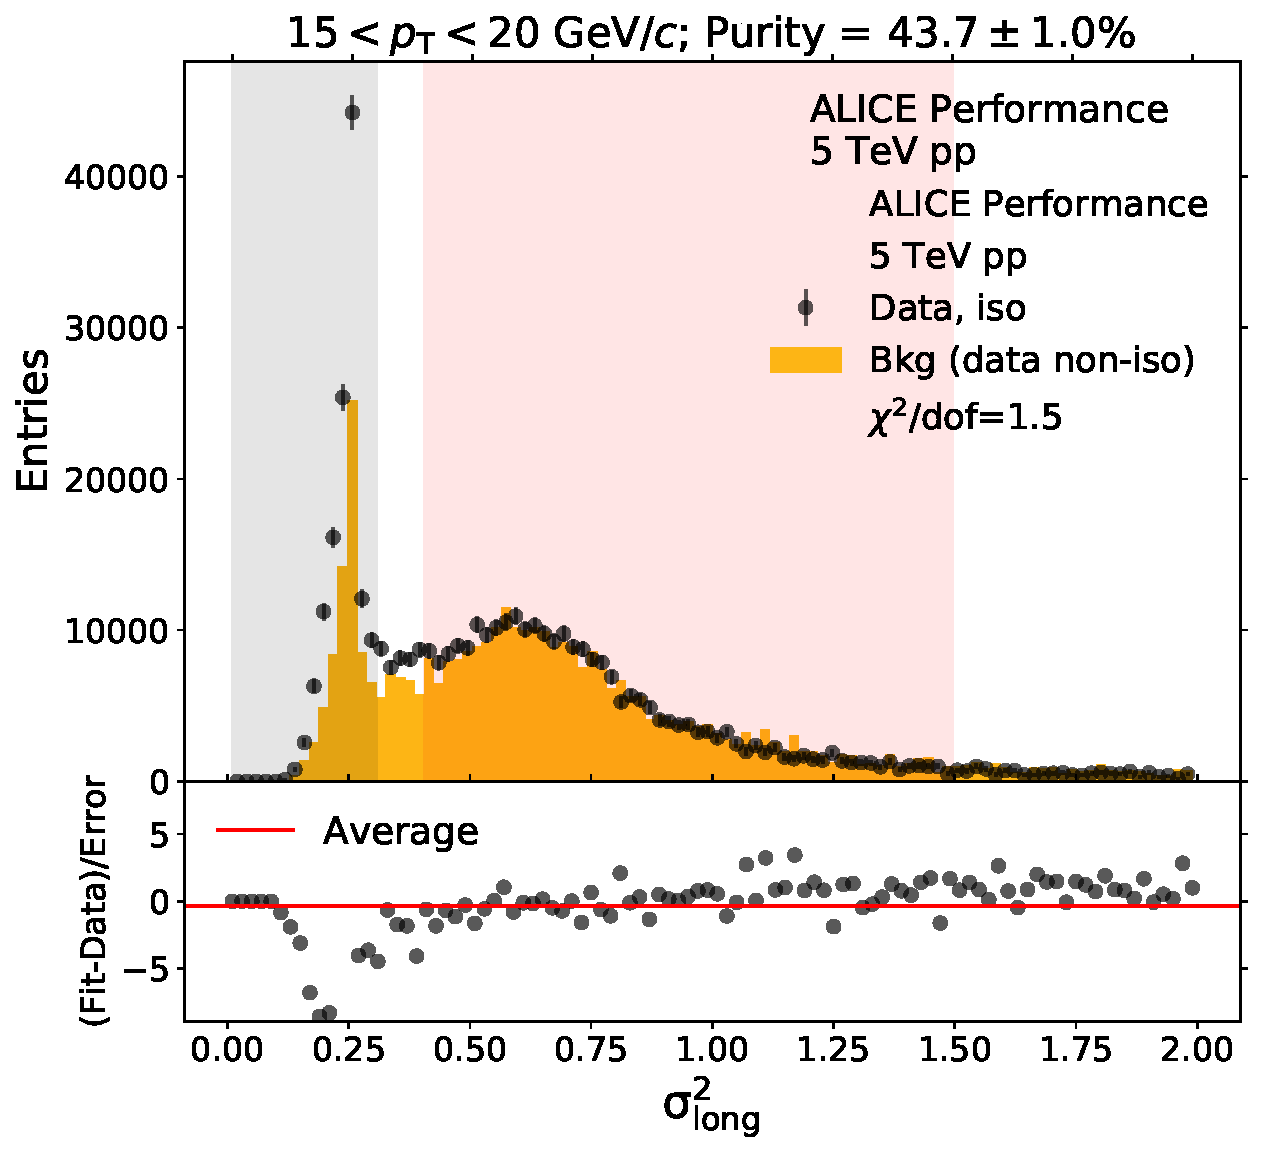
\includegraphics[width=0.38\textwidth]{Purity/bf-example-pp-cluster_Lambda-15-20.pdf}
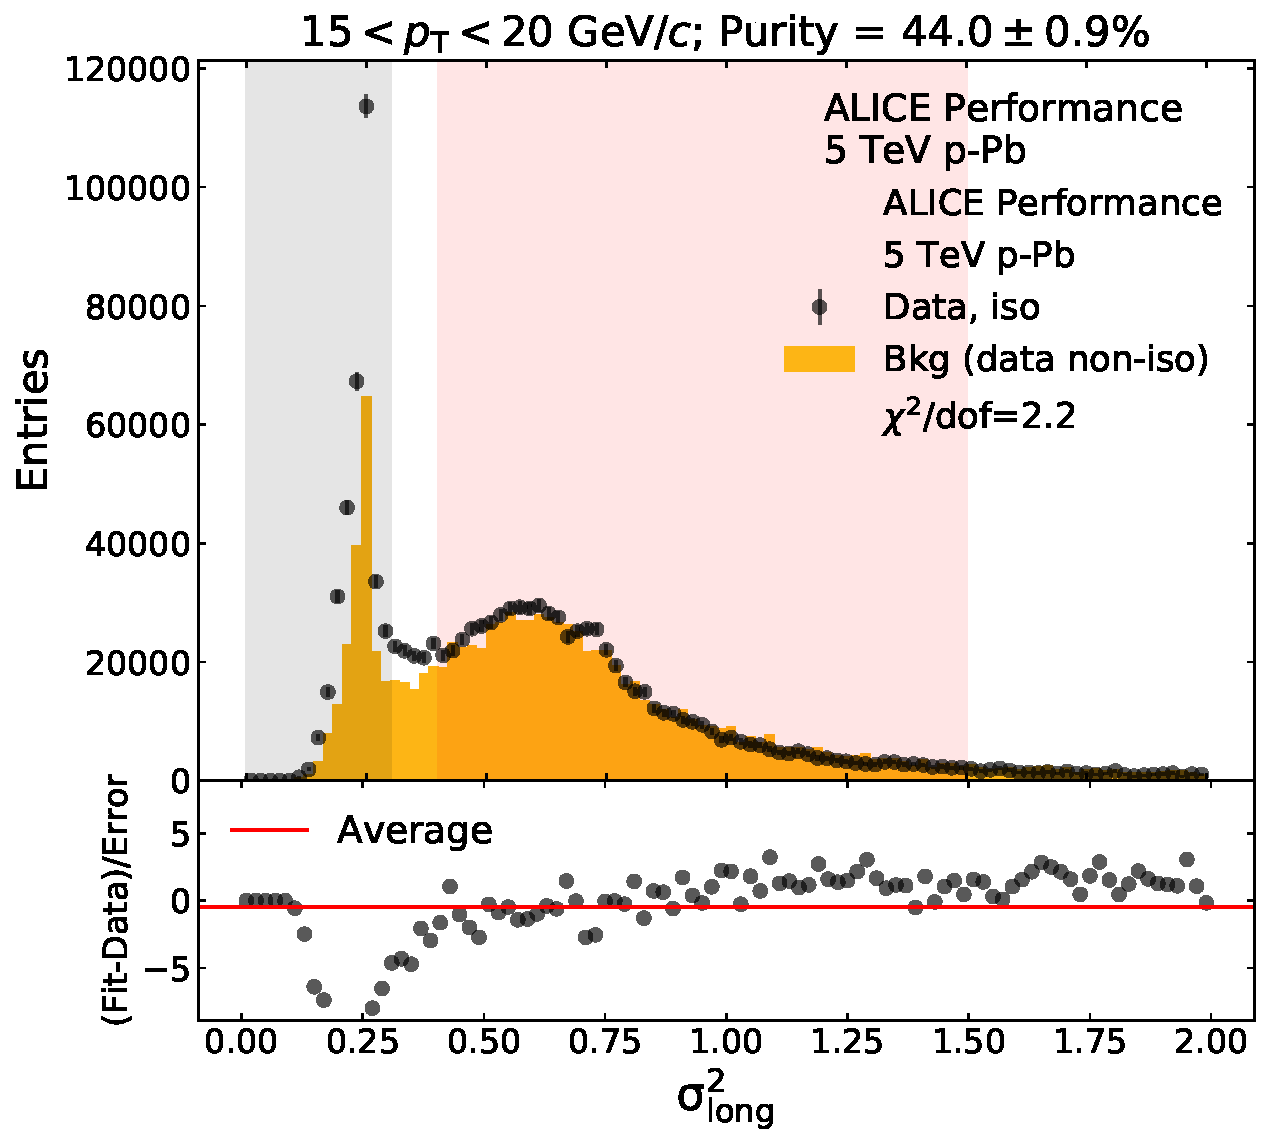
\includegraphics[width=0.38\textwidth]{Purity/bf-example-p-Pb-cluster_Lambda-15-20.pdf}
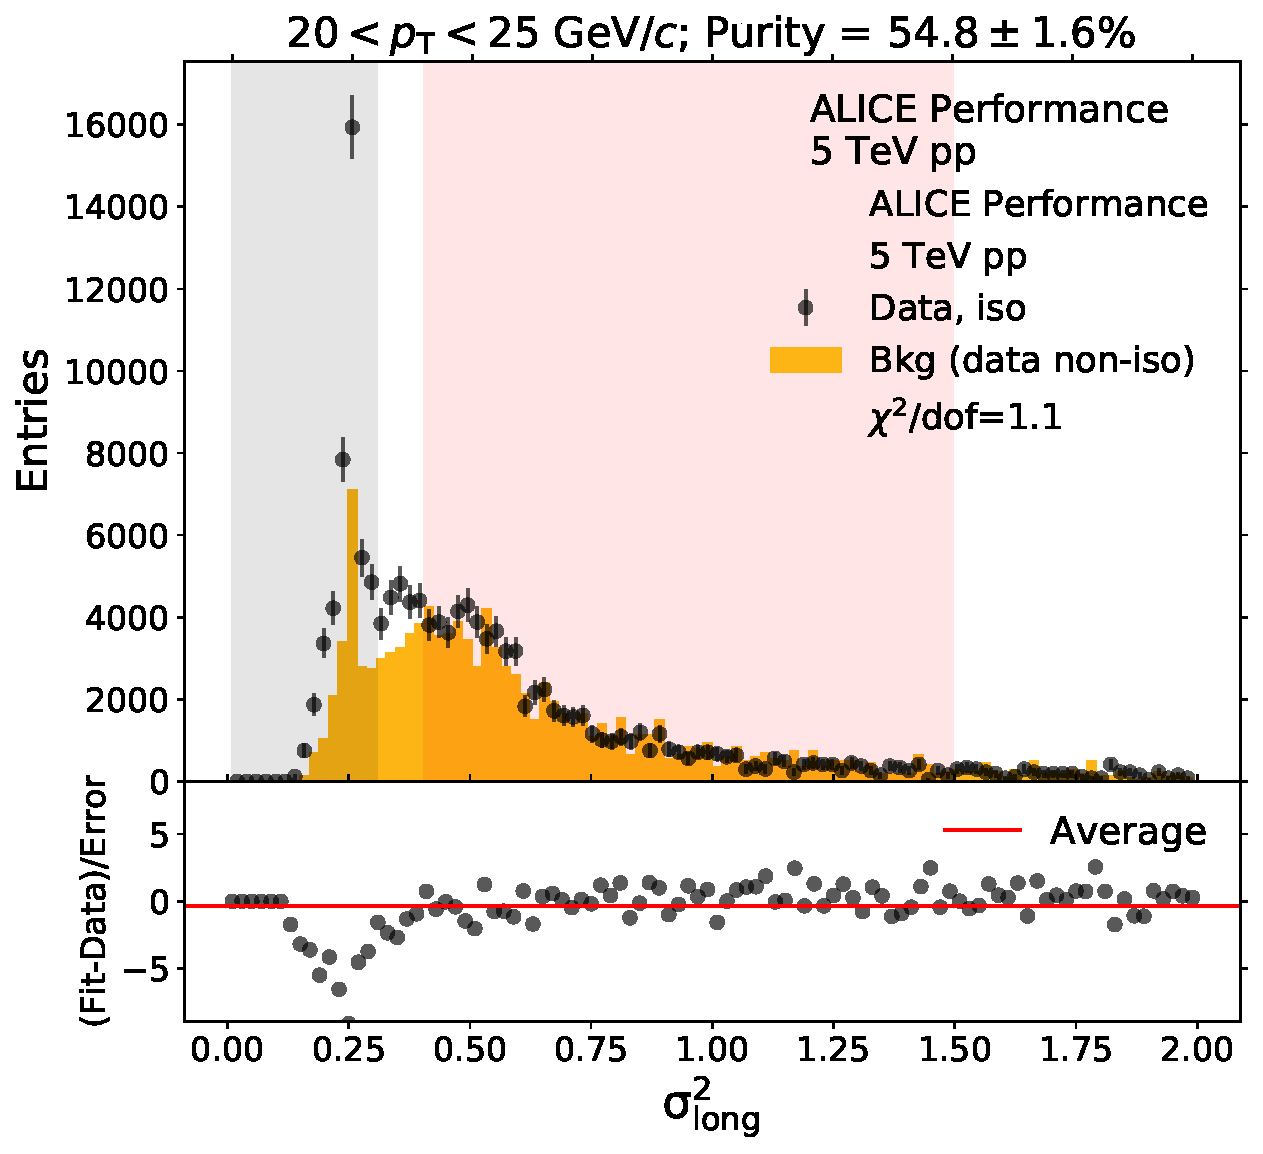
\includegraphics[width=0.38\textwidth]{Purity/bf-example-pp-cluster_Lambda-20-25.pdf}
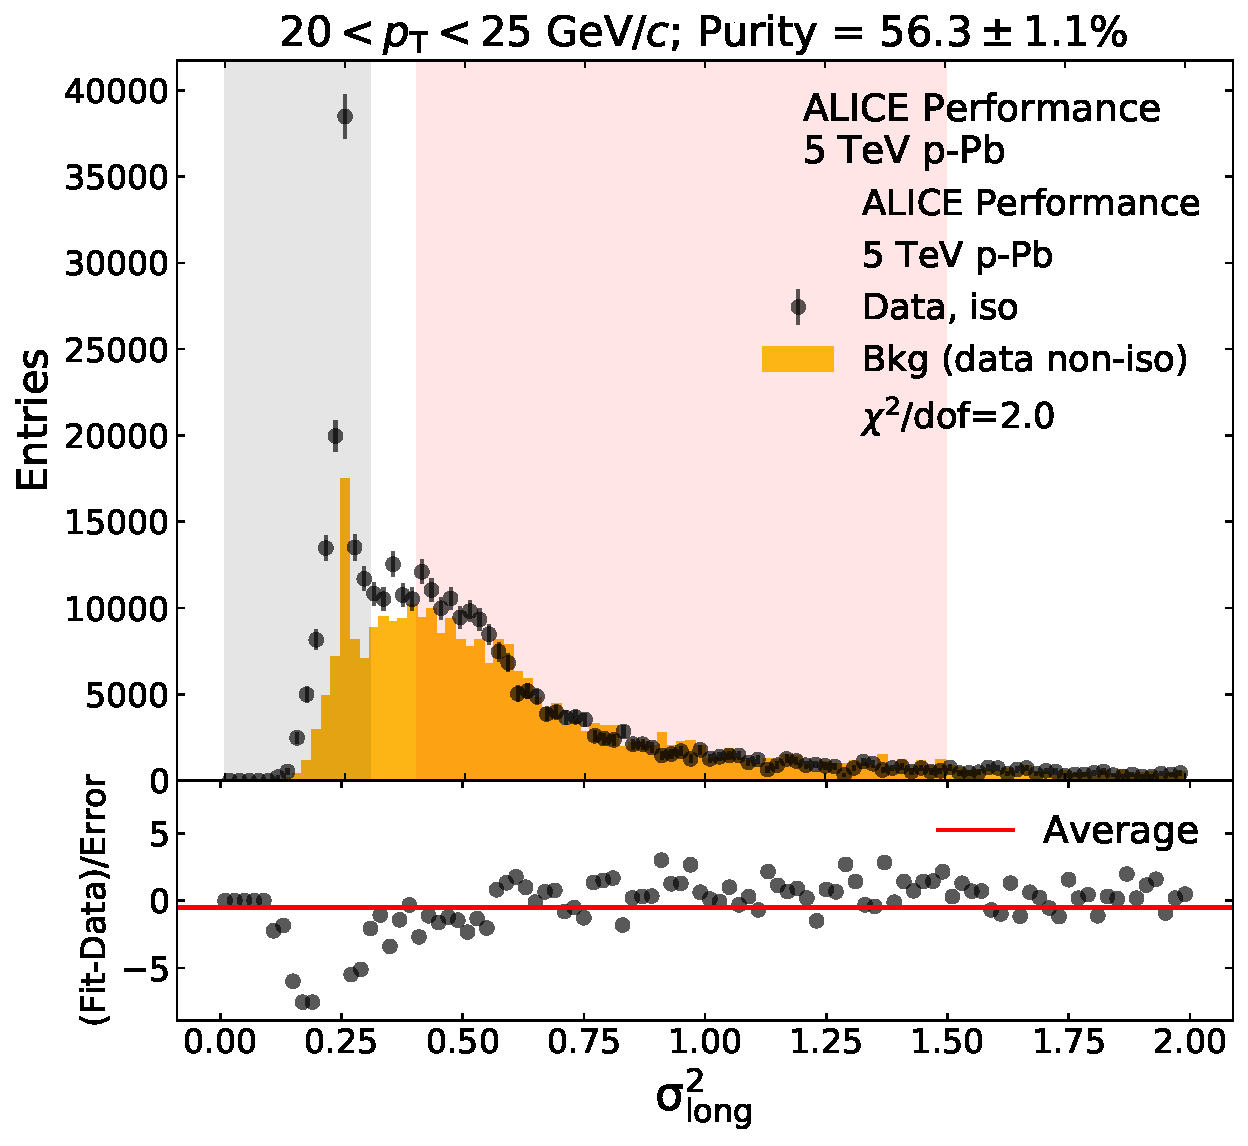
\includegraphics[width=0.38\textwidth]{Purity/bf-example-p-Pb-cluster_Lambda-20-25.pdf}
\\
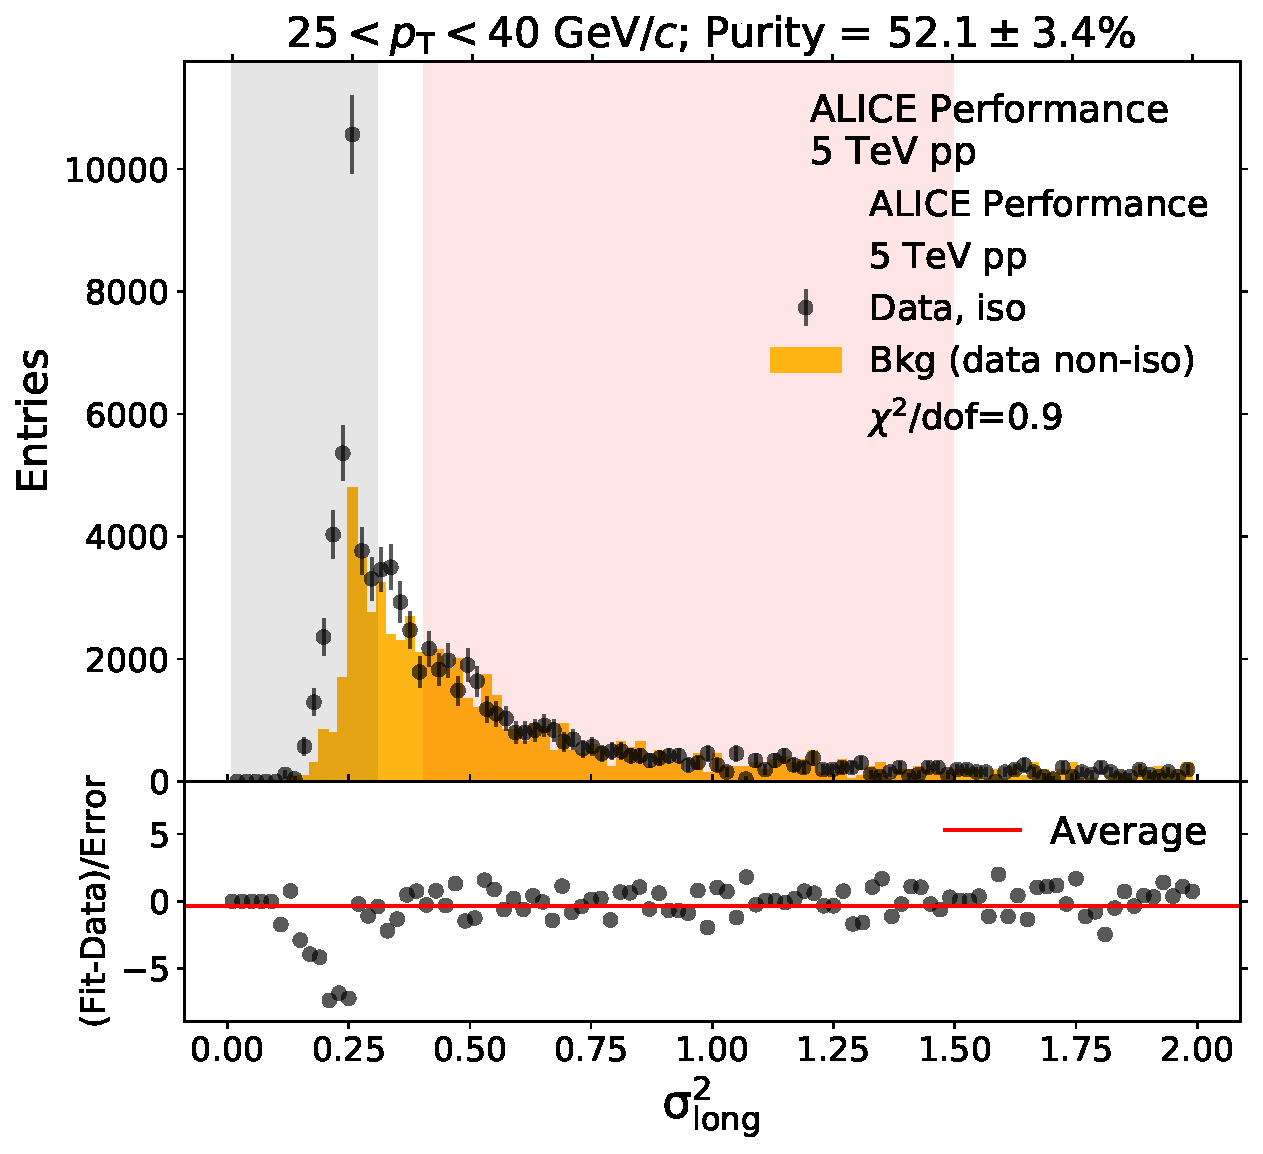
\includegraphics[width=0.38\textwidth]{Purity/bf-example-pp-cluster_Lambda-25-40.pdf}
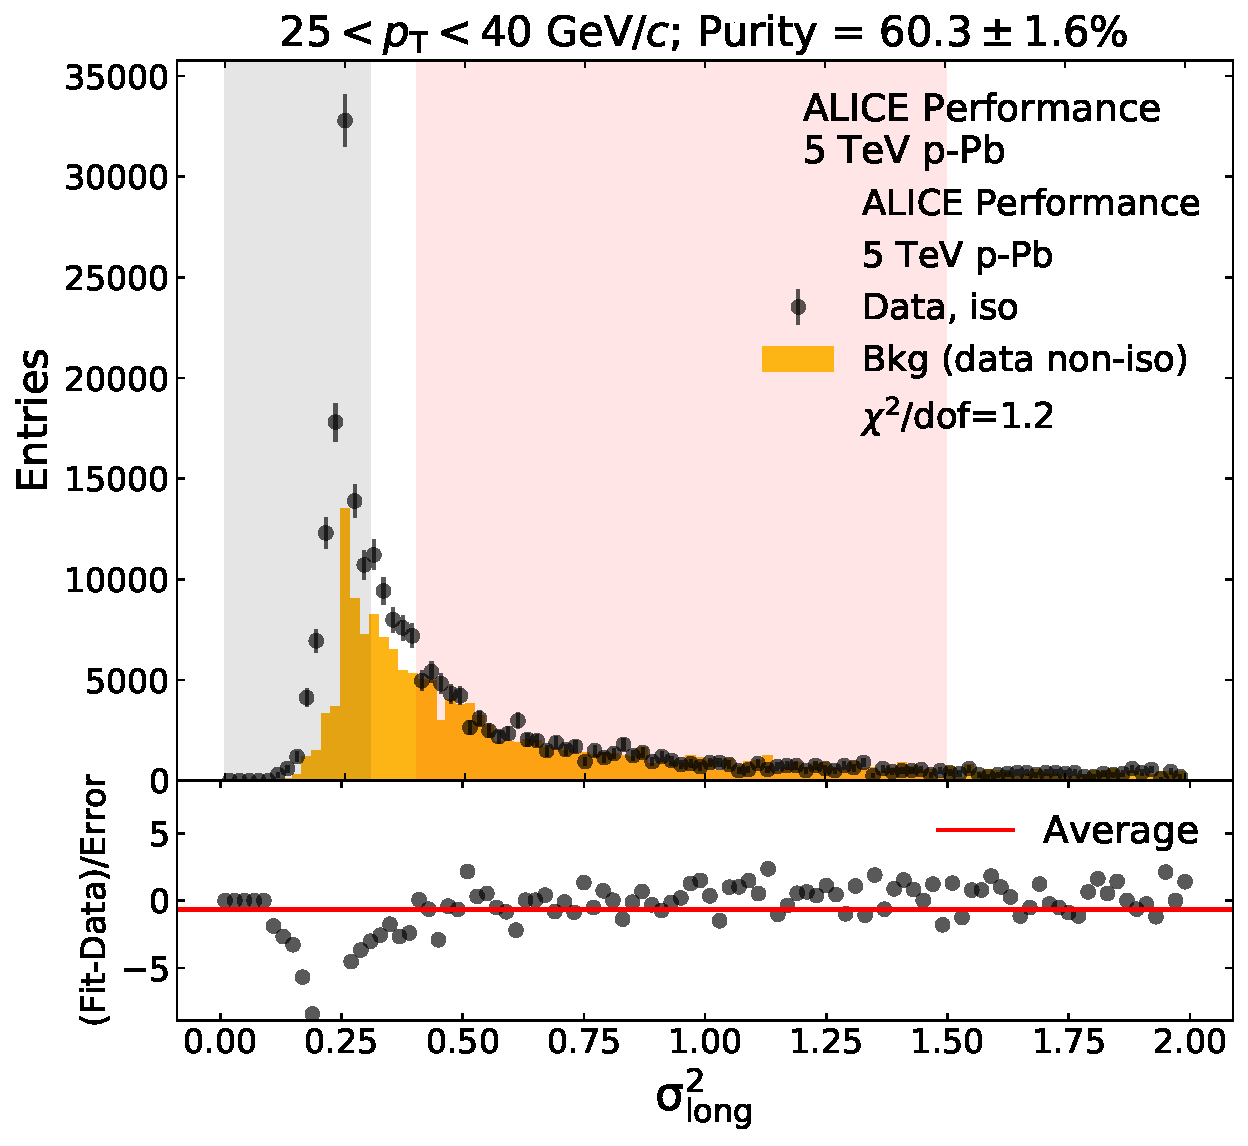
\includegraphics[width=0.38\textwidth]{Purity/bf-example-p-Pb-cluster_Lambda-25-40.pdf}
\caption{Template fit results of background-only template method for pp and \pPb~data. The yellow histograms are the predicted counts given the best-fit value of the total number of clusters in the background dominated region. The hatched gray area represents the interval considered for the purity estimate. The bottom panels show the normalized residuals of the fit, considering the statistical uncertainty on the isolated data and the background template added in quadrature. }
\label{BkgOnlyFit_pPb}
\end{figure}

This method makes the additional assumption that the fraction of signal misclassified as background is small. In a strict sense, this method yields a lower limit on the extracted purity. The results agree with our nominal results within a few percent, indicating that we are not particularly sensitive to the details of the modeling of the shower shape. As a conservative estimate, we take the full difference between our nominal results as a systematic uncertainty in the signal template.

As an additional check, we smear the signal template by multiplying the $\lambdasquare$ of each cluster by a random number selected from a Gaussian with a fixed width before then calculating the purity with this smeared distribution. This was done for a variety of widths up to 10\%, which is much larger than the expected MC simulation mismodelling, and was found to yield a smaller uncertainty than the background-only fit (See Appendix~\ref{sec:smearingsignaltemplate} for more details). Thus, for a final estimate of the systematic uncertainty from the signal template, we take the uncertainty estimated by the background-only fits as described in the previous paragraph.

\FloatBarrier
\subsubsection{Sideband variation in the background template}
\label{sec:bkgtemplate}
To estimate the shower-shape distribution for the $\ydecay$ background in the template fit, a sideband in the cluster isolation variable is used. Only the shape of this distribution is relevant, as the overall background normalization in the signal region (i.e. the purity) is measured with the template fit. As in any analysis using a sideband technique, we nominally use a sideband as close as possible to the signal region and as narrow as possible. Here, we describe how the sideband region is chosen and address the systematic uncertainty that arises from this arbitrary choice.

The cluster isolation distribution is divided into narrow (2 \GeVc) overlapping regions, each of which is used to estimate the background shower-shape distribution. A template fit is performed with each distribution and the $\chi^2$/dof and purity are calculated for each fit and plotted as a function of the anti-isolation region used to create the background template in Figure~\ref{sidebandslices}. Then, the $\chi^2$/dof distribution is examined to determine which regions of anti-isolation result in good fits in the template fit procedure: 5--10 \GeVc~is chosen to be the sideband definition in the final purity calculation.

To calculate the systematic uncertainty on the purity due to this selection, the full range of purities reached by the narrow bands of anti-isolation that fall within 5--10 \GeVc~is considered. Converting the full extent to a systematic uncertainty is a matter of dividing by $\sqrt{12}$ (i.e, the 1 $\sigma$ for a uniform distribution). This results in an absolute uncertainty on the purity of 0.7--5.8$\%$, depending on the collision system and cluster \pt~range.

\begin{figure}[h]
\center
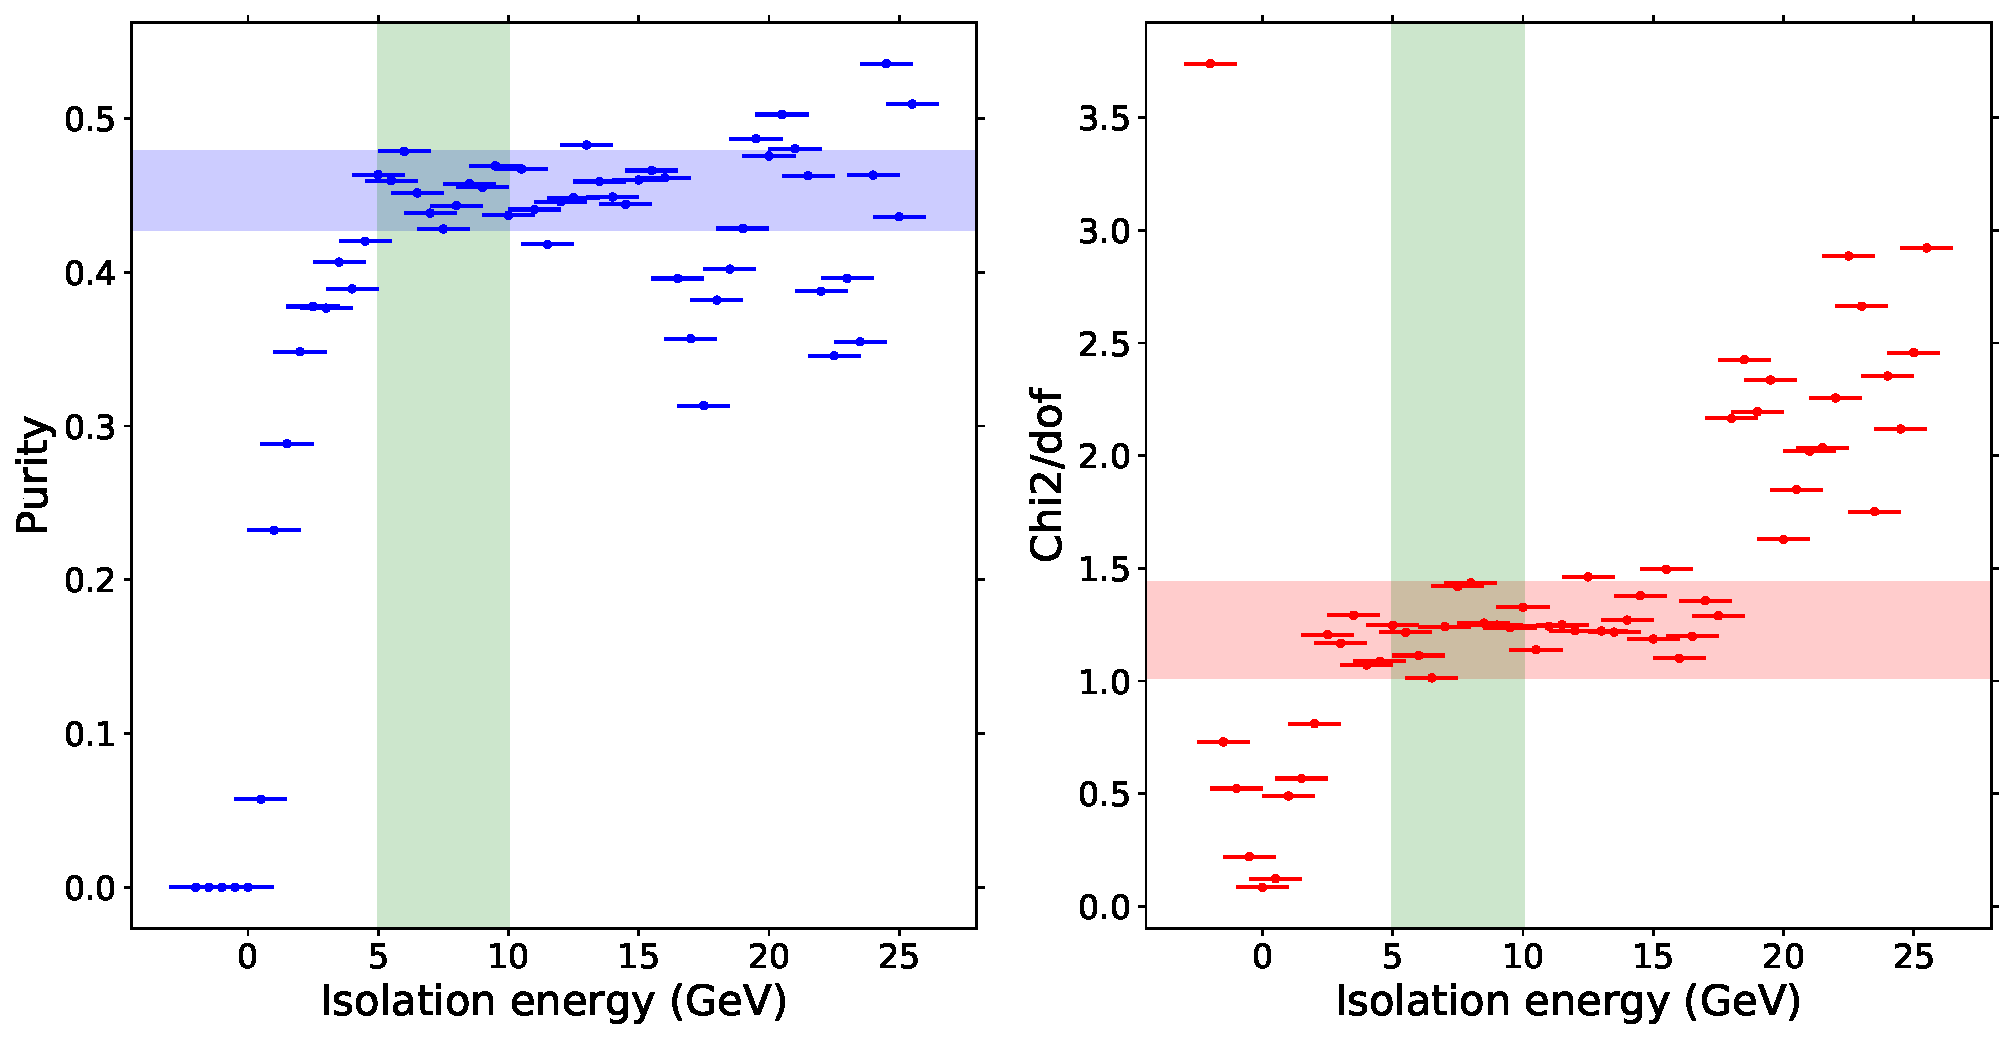
\includegraphics[width=1.0\textwidth]{Purity/antiiso-selection-pp-cluster_Lambda-15-20.pdf}\\
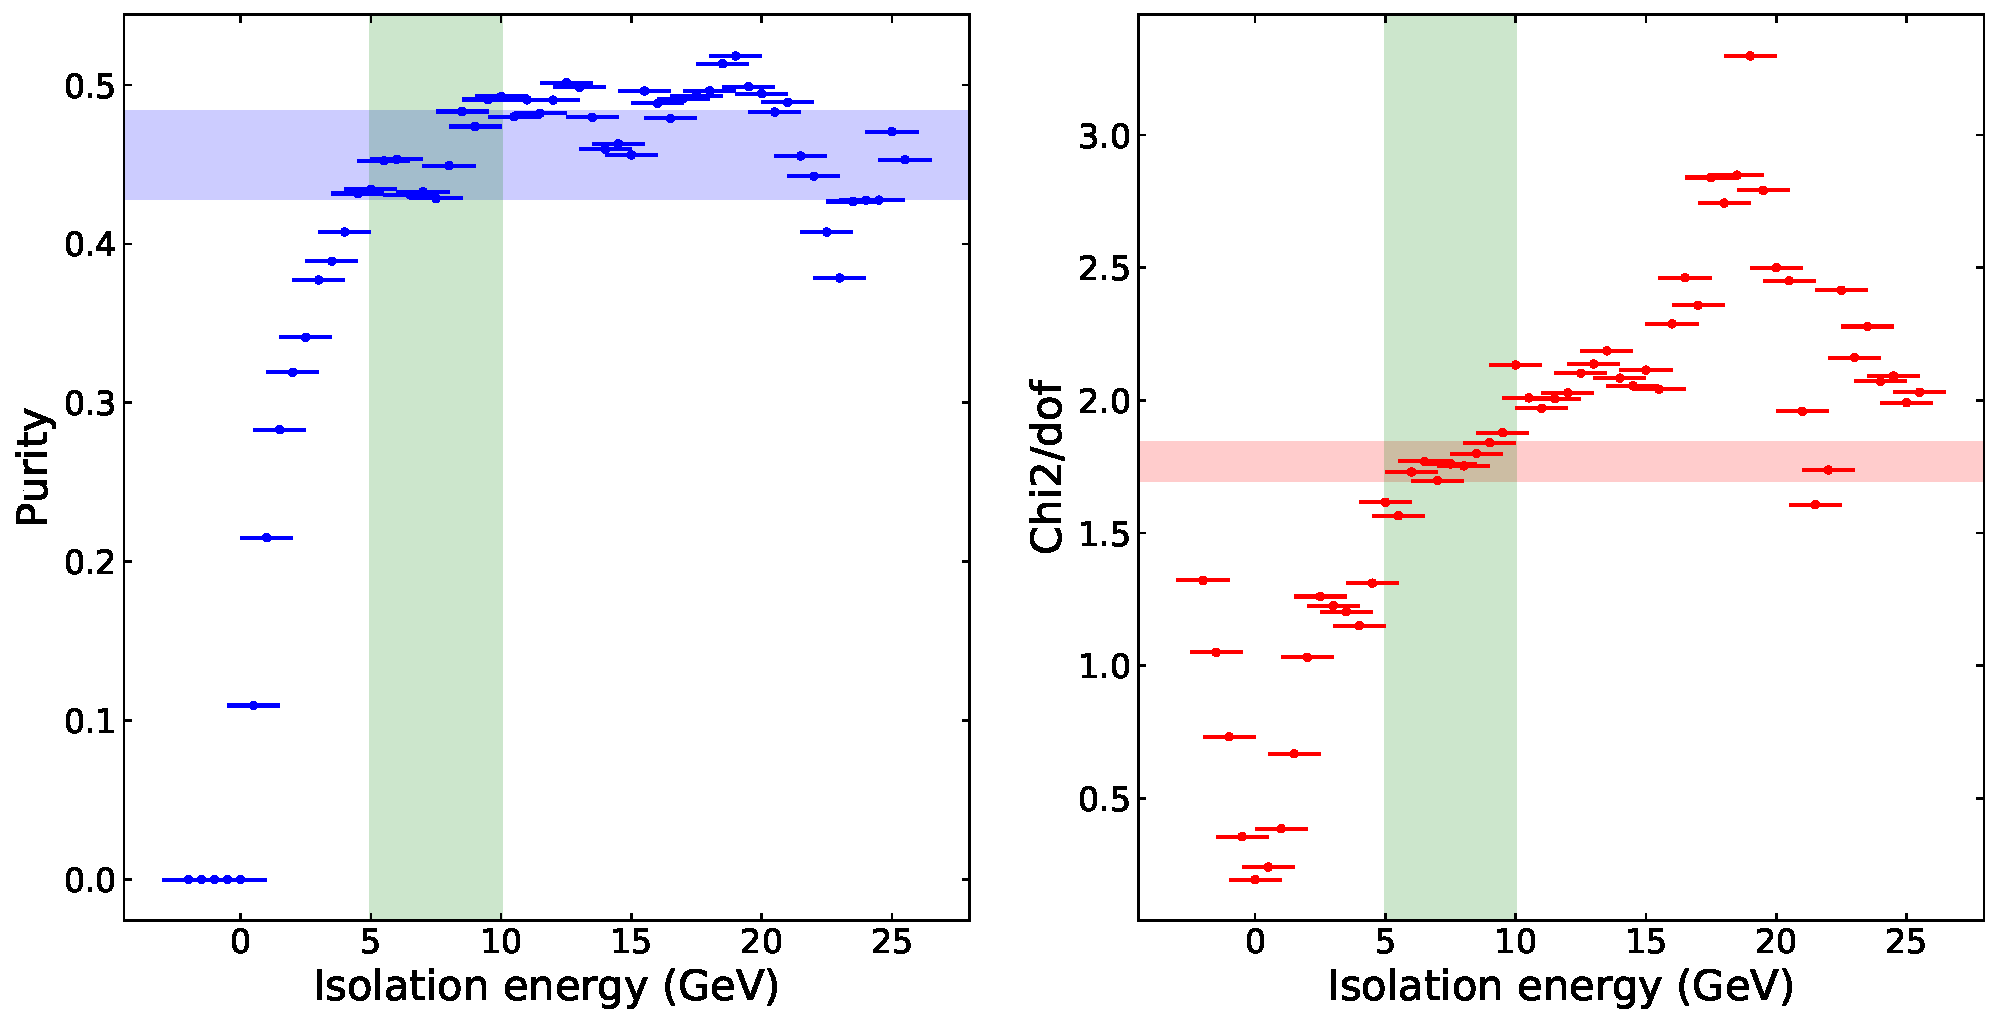
\includegraphics[width=1.0\textwidth]{Purity/antiiso-selection-p-Pb-cluster_Lambda-15-20.pdf}
\caption{Template fit results (purity and $\chi^2$/dof) as a function of anti-isolation region for clusters with $15 < \pt < 20$ \GeVc~in pp (top) and \pPb~(bottom). The green band shows the selected sideband region. The blue and red bands show the full extent of the purity within the selected sideband region.}
\label{sidebandslices}
\end{figure}

\subsubsection{Background template correction}
\label{sec:bkgtemplatecorrection}
Due to the correlation between the isolation and shower shape, the template extracted from the anti-isolated sideband does not exactly reflect the shape of the background in the signal region. Clusters in the isolation sideband have more associated activity than those in the true isolated background and thus emphasize the non-signal region of the shower-shape distribution. Consequently, using the isolation sideband instead of the true isolated background yields systematically higher purities. We note that a similar observation was made for example by the CMS collaboration in their template-fit purity measurements (e.g. Ref.~\cite{Sirunyan:2017qhf})

We correct this bias using a dijet MC simulation, as described in Equation~\ref{eq:bkgtemplatecorrection}. However, this correction is only valid to the extent that the dijet MC reproduces the data. To estimate the systematic uncertainty on this correction, we use a technique based on a method used in the ABCD calculation~\cite{Erwann}. In particular, we use a double ratio to check to which extend does the dijet MC describe the background-dominated region in data: 

\begin{equation}
    \text{Double ratio} = \frac{\text{Iso}_{\text{data}}/\text{Anti-iso}_{\text{data}}}{\text{Iso}_{\text{MC}}/\text{Anti-iso}_{\text{MC}}}
    \label{eq:bkgtemplatedoubleratio}
\end{equation}

In the signal region of the shower shape distribution (0.0--0.3 for $\lambdasquare$), this double ratio will be far from unity, as the data have prompt photons and the dijet MC do not. However, away from that region, where background dominates, the double ratio should be flat (i.e. have no slope) if the dijet MC reproduces the background shower-shape of the data. We note that for this analysis only the shape is important and overall normalization is irrelevant. At a minimum, we expect the variation in the double ratio to be smooth. Thus we fit the double ratio to smooth functions (linear and exponential) in a shower shape range away from the signal region and extrapolate the fit back into the signal region. A similar procedure was used isolated-photon purity measurements with the ABCD method~\cite{Acharya:2019jkx,Erwann}.

Fits to the double ratio are shown in Figures~\ref{fig:bkgtemplatedoubleratiofits_pp} and~\ref{fig:bkgtemplatedoubleratiofits_pPb}, for pp and \pPb~data respectively. We found that the linear and exponential fits gave nearly identical results. In particular, the slope was sufficiently small that the higher-order terms in the exponential were negligible. Thus for the purposes of estimating the systematic uncertainty due to the background template correction, we chose to do only linear fits to the double ratio. In order to remove covariance effects between the slope and intercept, the fits were forced to go through the weighted average of the double ratio value within the fit range at the center of the fit range, making it a single-parameter linear fit with only the slope as a free parameter. This allowed us to propagate the fit uncertainty on the slope to an uncertainty on the purity.


\begin{figure}
    \centering
    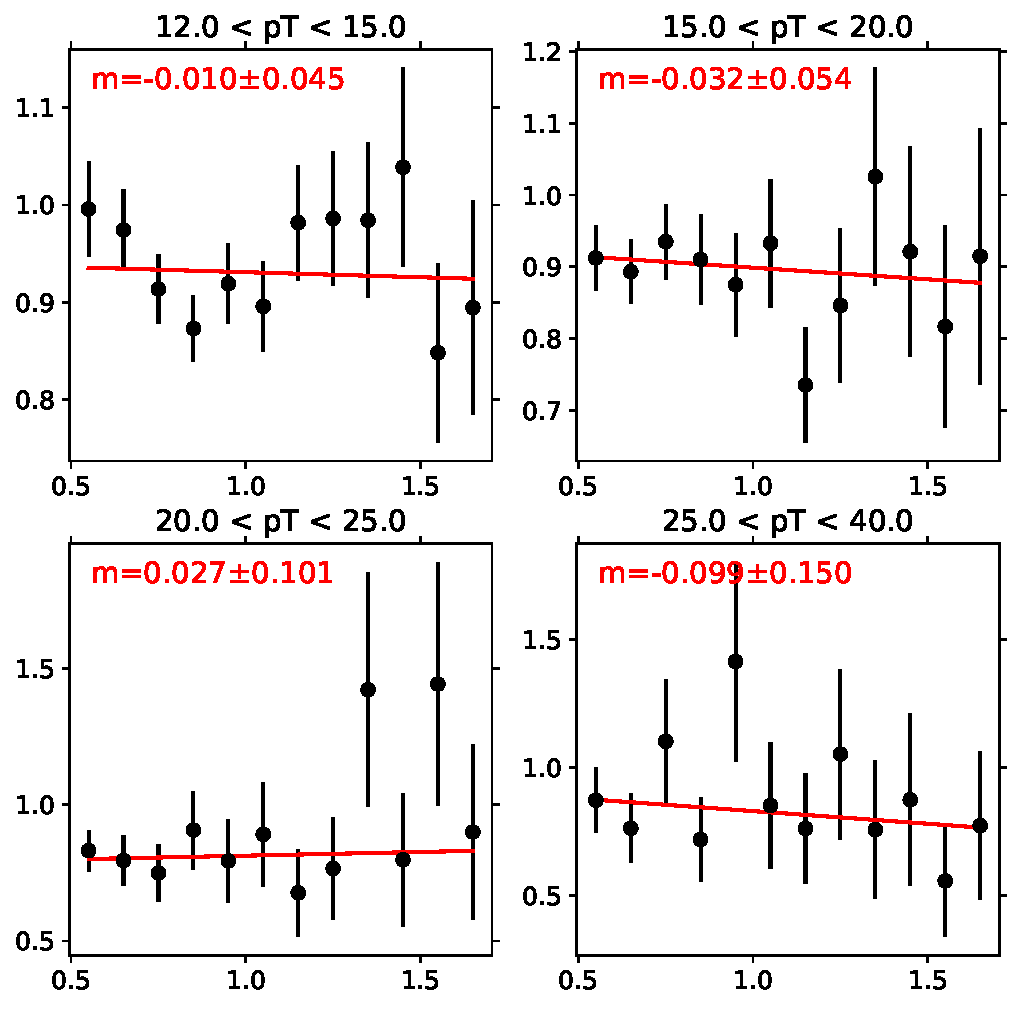
\includegraphics[width=\textwidth]{Purity/single-linear-fits-pp}
    \caption{Linear fits for the double ratio (as described in Equation~\ref{eq:bkgtemplatedoubleratio}) for the $\lambdasquare$ variable in pp data.  Included are the value and uncertainty of the fitted slope (in red).}
    \label{fig:bkgtemplatedoubleratiofits_pp}
\end{figure}


\begin{figure}
    \centering
    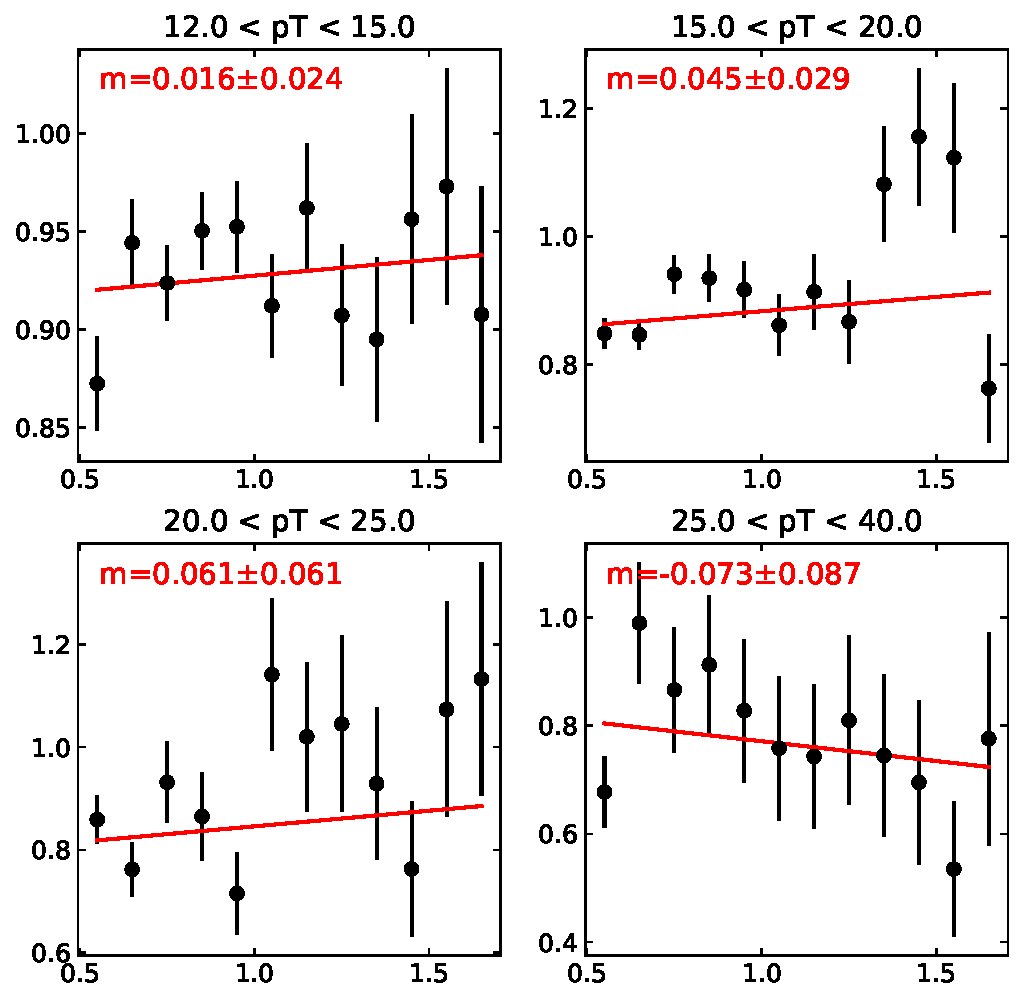
\includegraphics[width=\textwidth]{Purity/single-linear-fits-p-Pb}
    \caption{Linear fits for the double ratio (as described in Equation~\ref{eq:bkgtemplatedoubleratio}) for the $\lambdasquare$ variable in \pPb~data.  Included are the value and uncertainty of the fitted slope (in red).}
    \label{fig:bkgtemplatedoubleratiofits_pPb}
\end{figure}







These linear fits to the double ratio were done in two fit ranges: 0.5--1.5 and 0.5--1.75 for $\lambdasquare$. In all cases, we found that the slopes were consistent with 0 within the fit uncertainties and thus concluded that that the dijet MC was consistent with the data. Therefore, we did not apply an additional double-ratio correction to the Weights function in Equation~\ref{eq:bkgtemplatecorrection}. We also found that the double ratio fits with the different fit ranges gave purities consistent with each other. So in order to minimize the amount of extrapolation, we did the fit in the largest reasonable fit ranges for each of the variables (the larger of each of the ranges described at the beginning of this paragraph). 

We then took the uncertainty on that double ratio fit and propagated it to a purity uncertainty. This purity uncertainty was then taken to be the systematic uncertainty on the background correction. It varies between 1.2--3.4\% (absolute) depending on cluster \pt~and collision system.


\FloatBarrier
%%%%%%%%%%%%%%%%%%%%%%%%%%%%%%%%%%%%%%%%%%%%%%%%%%%%%%%%%
\subsection{Summary of systematic uncertainties of purity measurement}

Tables~\ref{tab:pursystppblambda} and~\ref{tab:pursystpplambda} give the full estimates of the systematic uncertainties in both collision systems. No single source of systematic uncertainty dominates across \pt~ranges or collision systems.


\begin{table}[h]
    \centering
        \caption{Summary of the systematic uncertainties on the purity as measured with $\lambdasquare$ in \pPb~collisions. All values are in absolute percentage. ``Stat.'' refers to the statistical uncertainty; ``Signal'' refers to the signal template uncertainty; ``Anti-iso'' refers to the uncertainty due to the sideband selection; ``Bkg'' refers to the uncertainty due to the background template correction; ``Total'' is the sum of the previous three columns in quadrature.}
    \begin{tabular*}{1.0\columnwidth}{@{\extracolsep{\fill}}lcccccc@{}}
    \hline
    	pT(GeV/$c$) & Purity & Stat. & Signal & Anti-iso & Bkg & Total syst \\ \hline
    	12.0-15.0 & 20.7 & 1.1 & 1.1 & 0.8 & 1.5 & 2.0 \\
    	15.0-20.0 & 34.2 & 1.2 & 2.0 & 1.6 & 1.2 & 2.8 \\
    	20.0-25.0 & 47.6 & 1.7 & 1.9 & 1.1 & 1.7 & 2.7 \\
    	25.0-40.0 & 54.6 & 1.8 & 2.3 & 2.4 & 2.1 & 3.9 \\
    \end{tabular*}
    \label{tab:pursystppblambda}
\end{table}


\begin{table}[h]
    \centering
        \caption{Summary of the systematic uncertainties on the purity as measured with $\lambdasquare$ in pp collisions. All values are in absolute percentage. ``Stat.'' refers to the statistical uncertainty; ``Signal'' refers to the signal template uncertainty; ``Anti-iso'' refers to the uncertainty due to the sideband selection; ``Bkg'' refers to the uncertainty due to the background template correction; ``Total'' is the sum of the previous three columns in quadrature.}
    \begin{tabular*}{1.0\columnwidth}{@{\extracolsep{\fill}}lcccccc@{}}
    \hline
    	pT(GeV/$c$) & Purity & Stat. & Signal & Anti-iso & Bkg & Total syst \\ \hline
    	12.0-15.0 & 20.1 & 1.7 & 2.0 & 1.2 & 2.9 & 3.7 \\
    	15.0-20.0 & 31.7 & 2.0 & 2.5 & 1.5 & 2.4 & 3.8 \\
    	20.0-25.0 & 47.3 & 2.9 & 0.8 & 3.0 & 2.8 & 4.2 \\
    	25.0-40.0 & 48.5 & 3.5 & 5.9 & 4.0 & 3.4 & 7.9 \\
    \end{tabular*}
    \label{tab:pursystpplambda}
\end{table}


%[I have commented out, it is redundant]
%An overall summary of the purity, statistical uncertainty, and total systematic uncertainty in pp and \pPb~datasets is given in Table~\ref{tab:puruncertaintypp}.

%\begin{table}[h]
%	\centering
%		\caption{Summary of purities and statistical and systematic uncertainties for pp and \pPb~collisions. All values are absolute percentages.}
    % \begin{tabular*}{1.0\columnwidth}{@{\extracolsep{\fill}}l|ccc|ccc@{}}
    % 	\hline
    % 	 & \multicolumn{3}{c|}{pp} & \multicolumn{3}{c}{p-Pb} \\ \hline
    % 	pT(GeV/$c$) & \lambdasquare & $\sigma_{\text{stat}}$ & $\sigma_{\text{syst}}$ & \lambdasquare & $\sigma_{\text{stat}}$ & $\sigma_{\text{syst}}$ \\ \hline
    % 	12.0--15.0 & 20.1 & 1.7 & 3.7 & 20.7 & 1.1 & 2.0 \\
    % 	15.0--20.0 & 31.7 & 2.0 & 3.8 & 34.2 & 1.2 & 2.8 \\
    % 	20.0--25.0 & 47.3 & 2.9 & 4.2 & 47.6 & 1.7 & 2.7 \\
    % 	25.0--40.0 & 48.5 & 3.5 & 7.9 & 54.6 & 1.8 & 3.9 \\
    % 	\hline
    % \end{tabular*}
%	\label{tab:puruncertaintypp}
%\end{table}

%\subsubsection{Data-driven shower shape with eta decays}
%We study the shower-shape distribution for single photons from data by using $\eta$ decays obtained in the 13 %TeV pp data collected in 2016 and 2017. Pairs of photons with an invariant mass consistent with a $\eta$ decay are used. The signal-to-noise ratio is about XX. The background is estimated by using a two-sided sideband around the $\eta$ peak. The shower-shape distributions for photons with $p_{T}>8 $ GeV is shown in Figure~\ref{ShoweShape} and is compared with the distribution obtained from sgamma--jet .  The simulation is weighted such that it matches the $p_{T}$ distribution measured in the data. 
%\begin{figure}
%\center
%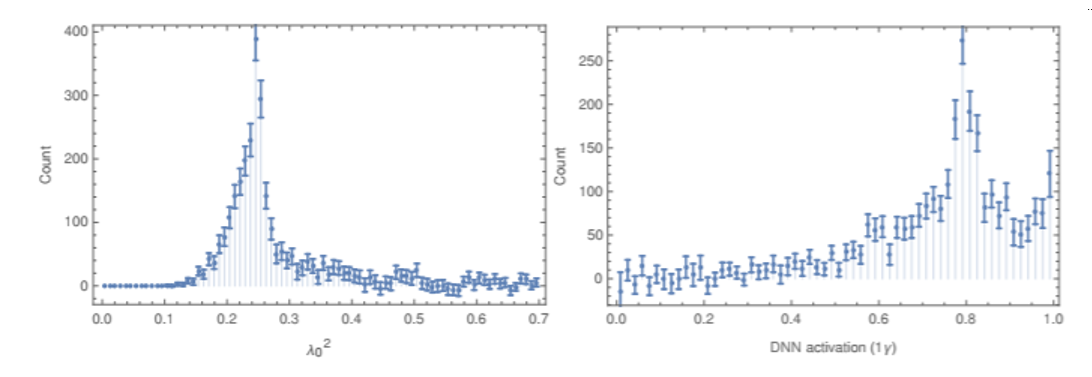
\includegraphics[width=0.95\textwidth]{Purity/EtaShowerShape}
%\caption{Data-driven shower shape (left panel is DNN and right panel lambda) distribution with photons from %$\eta$ decays. The simulation was weighted to reflect the $p_{T}$ distribution obtained in data}
%\label{ShoweShape}
%\end{figure}

%The comparison shows that the simulation is consistent with the data-driven distribution, within statistical uncertainties. 


%Figure~\ref{SignalShowerShapes} shows the distribution of the shower-shape variables for photon-jet simulation of pp collisions. The $\lambdasquare$ variable peaks at 0.25 and is mostly symmetric but has a small tail to larger values. The DNN variable shows a relatively broad peak at {DNN$\approx0.75$}, and a tail to lower values.
% The $\emax$ variables reveals that for most of the signal clusters the seeding cell contains about 75--85$\%$ of the total cluster energy, but the distribution has a pronounced tail that extends to values as low as 50$\%$ and an even smaller tail that reaches 25$\%$. 

%\begin{figure}[h]
%\center
%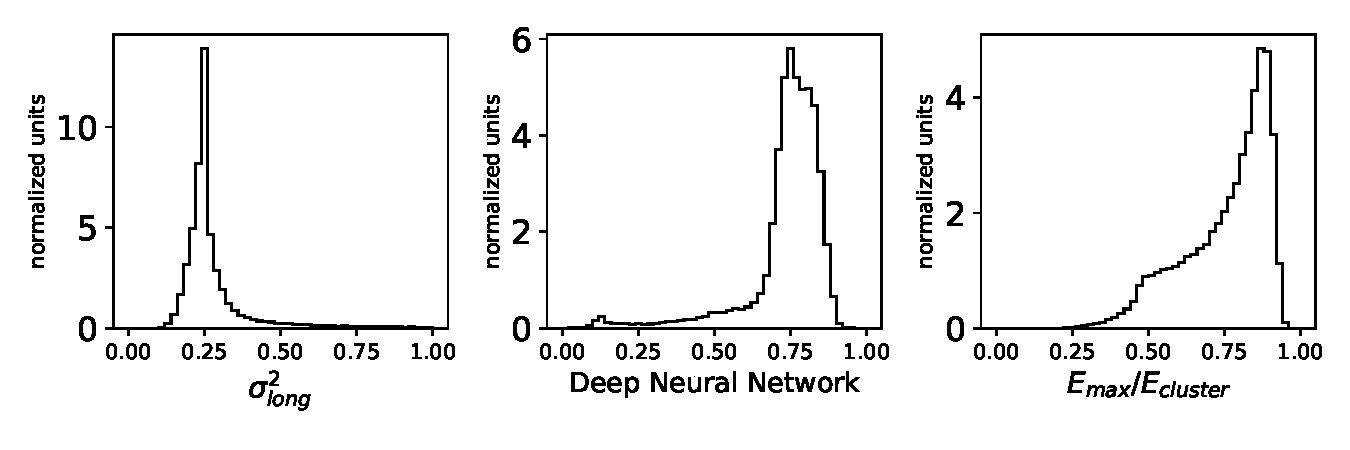
\includegraphics[width=1.0\textwidth]{Purity/ShowerShapeVariables}
%\caption{Shower shape distributions, from photon-jet simulation, of clusters with {$12<\pt<16$ GeV}.}
%\label{SignalShowerShapes}
%\end{figure}

%The shape of the distributions shown in Figure~\ref{SignalShowerShapes} reveal that not all the shower shapes from signal photons are similar (as a naive look at the $\lambdasquare$ peak would led us to believe). This is to be expected, as some photons hit near the center of a cell and the shower is contained in mostly one cell, while others hit near the boundary of cells, or hit at a slight angle due to the ``approximate protectiveness" of the EMCal/DCal system.

%FigureTemplatefitResults_pp shows fit results in p-Pb and pp data. In both cases, a good fit with no systematic pattern in the residuals is achieved over most of the distribution, with reduced $\chi^{2}$ in the 1.0--2.7 range. 
%The systematic variation of the residuals of the $\lambdasquare$ fit is attributed to the very sharp peak of this distribution. We do not attempt to further improve the fit quality but instead take these as part of our systematic uncertainties. In Section~\ref{sec:puritysystematics}, we also present results without a signal template. %The results show a signal fraction of about 10--13$\%$, integrated over the entire shower shape distributions. The purity is determined as the fraction to background after the shower shape cut that is used in the $\gammaiso$ selection (DNN$>0.55$ or $\lambdasquare<0.4$)

%\FloatBarrier
%\subsection{Consistency check with photon spectra}
%We perform a check on the purity and efficiency obtained with different shower-shapes on the number of prompt photons that pass our selection. The check is performed by correcting the spectrum of prompt photons passing the cuts by the cut efficiency and purity. The resulting spectra are then compared with one another. 
%The photon spectrum is a physical quantity that should be independent of the shower-shape cut used, so it allows us to cross-check the purity and shower-shape cut efficiency corrections. 

%Figure~\ref{fig:ShowerShapeEfficiency} shows the shower-shape cut efficiency. The $\lambdasquare<0.3$ and the DNN$>0.75$ selections yield similar efficiencies of about 80$\%$ with only a mild $\pt$ dependence.

%\begin{figure}[h]
%\center
%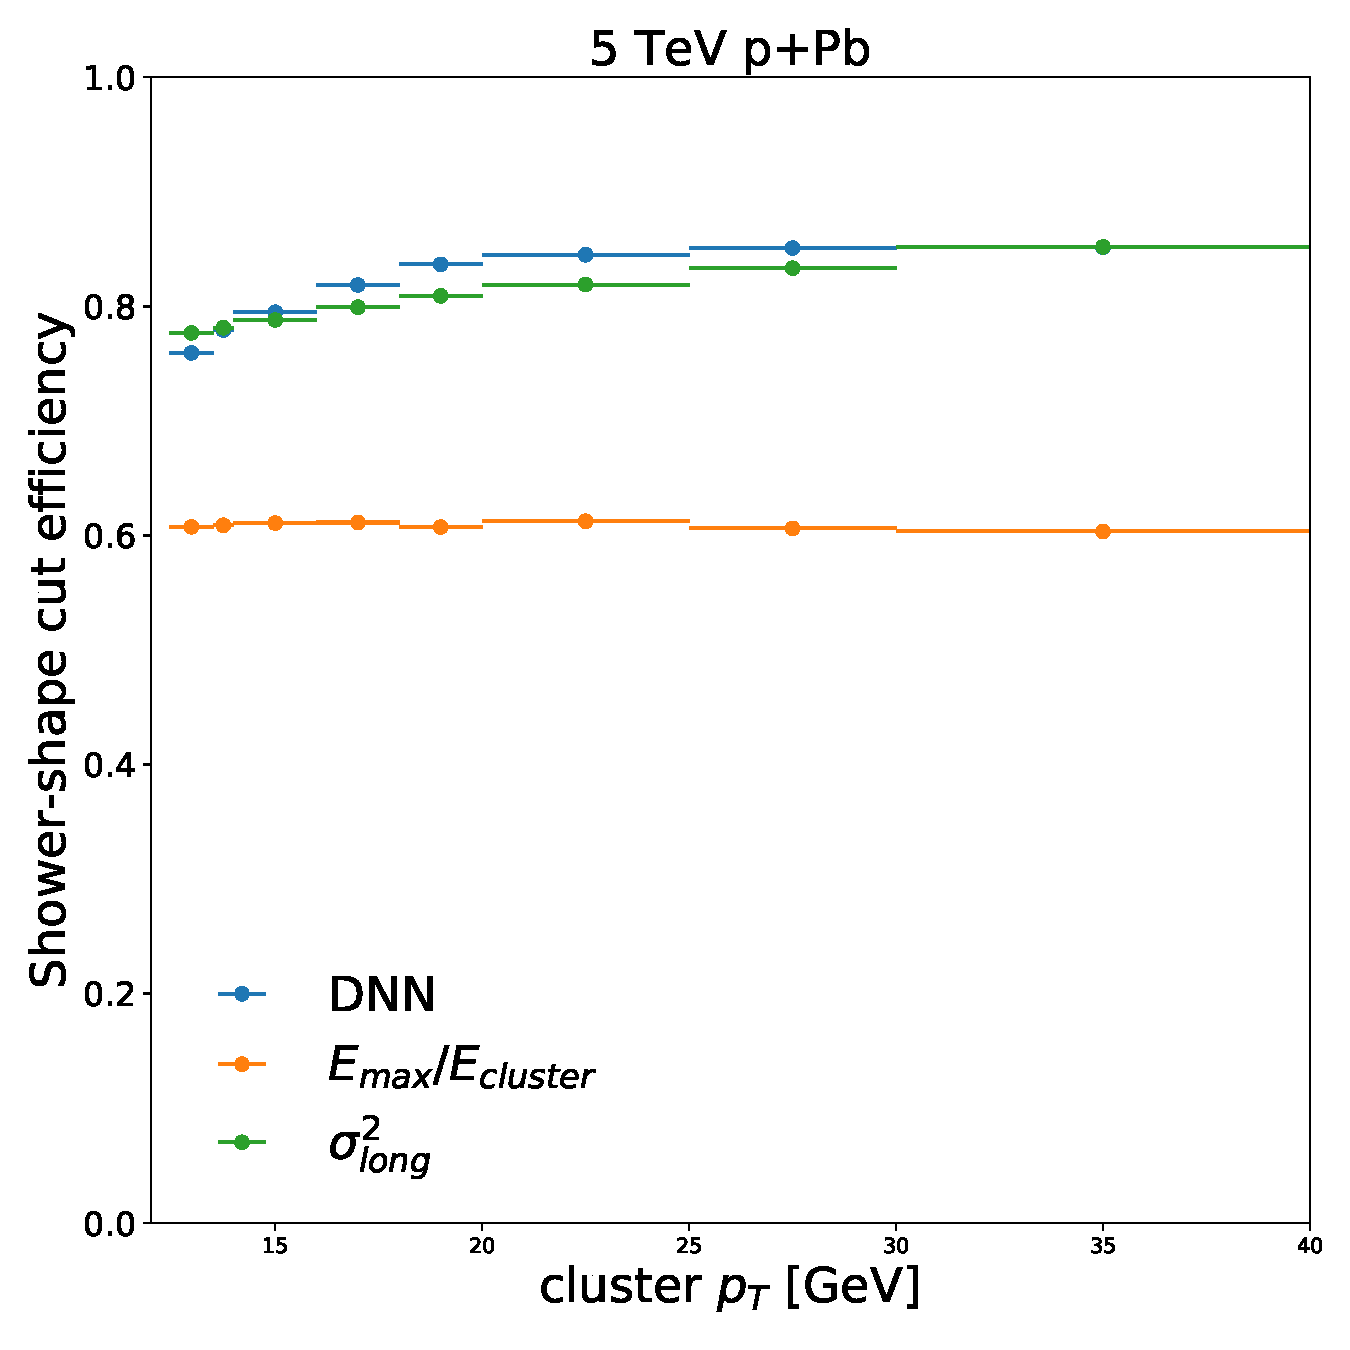
\includegraphics[width=0.495\textwidth]{Purity/ShowerShapeEfficiency_Skimmed_13def_root}
%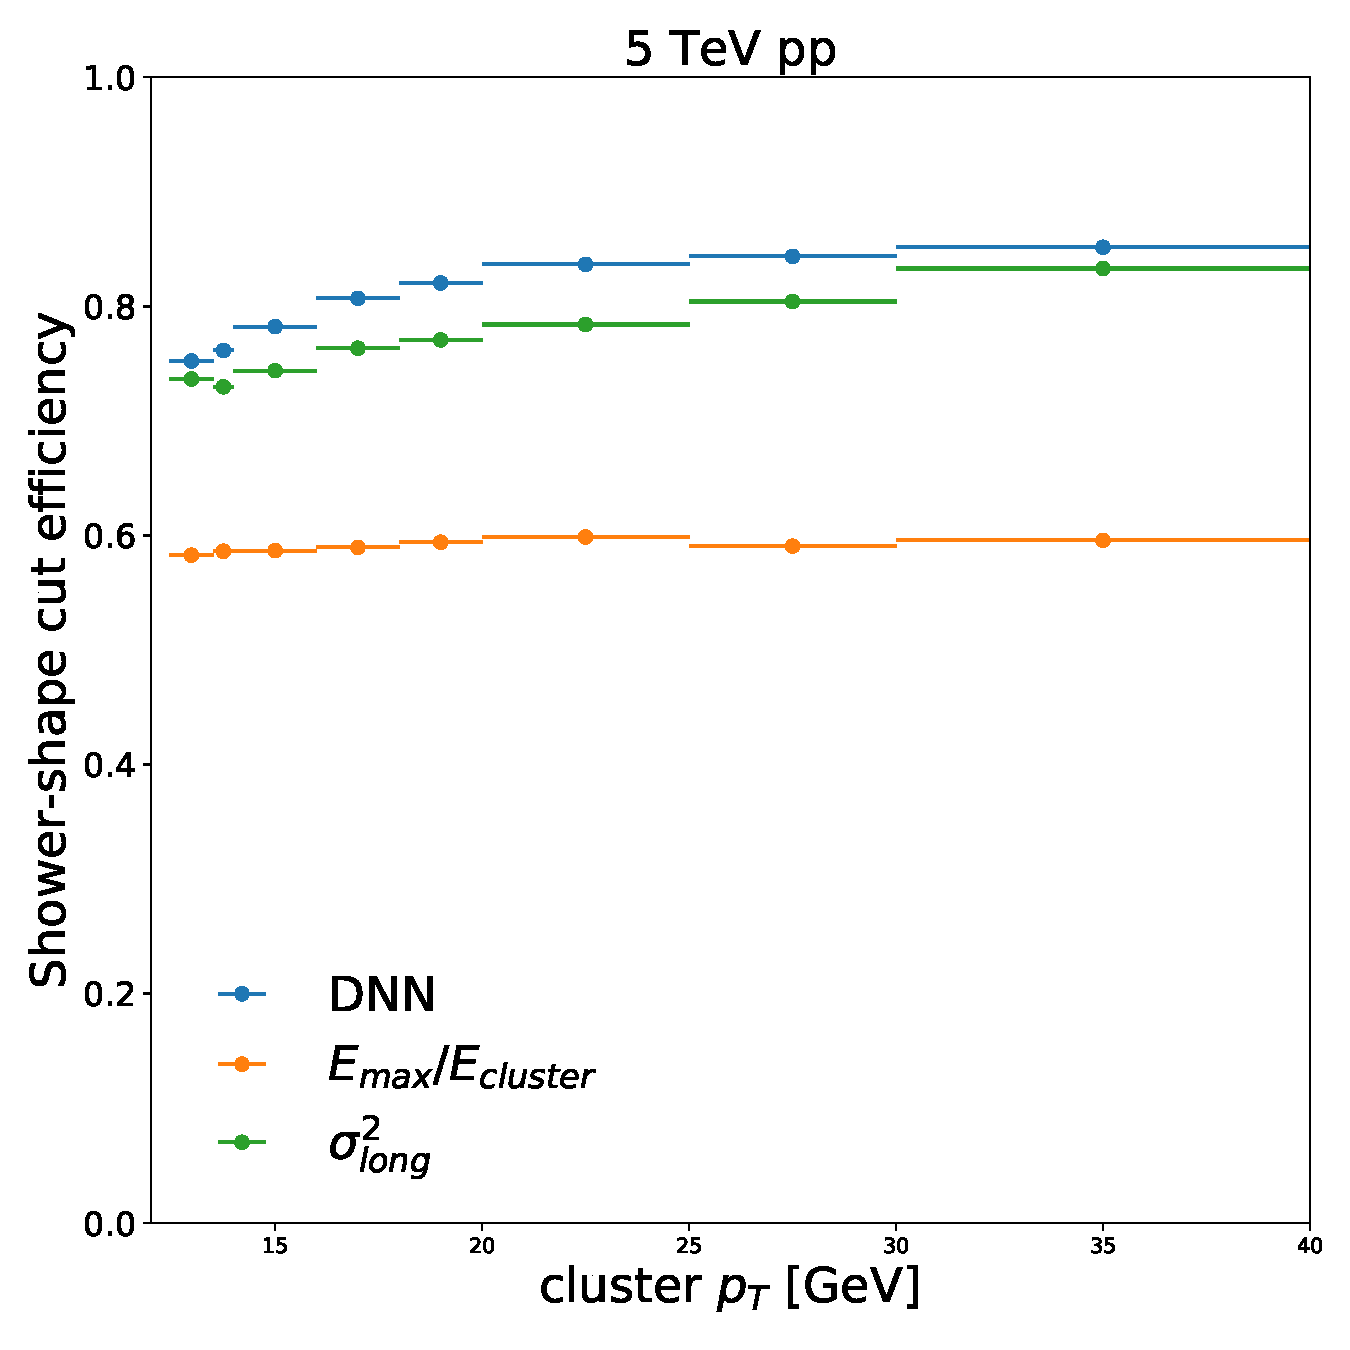
\includegraphics[width=0.495\textwidth]{Purity/ShowerShapeEfficiency_Skimmed_17q_root}
%\caption{Shower-shape cut efficiency as a function of cluster $\pt$ obtained from photon+jet simulations in p-Pb (left) and pp (right). The statistical uncertainty in the measurement is smaller than the marker size.}
%\label{fig:ShowerShapeEfficiency}
%\end{figure}

%Figure~\ref{fig:ConsistencywithSpectra} shows the results of the check in p-Pb and pp data. The obtained spectra are consistent within $15--20\%$ of the average over the momentum range measured. 

%\begin{figure}[h]
%\center
%\includegraphics[width=0.495\textwidth]{Purity/Spectra_Skimmed_13def_root}
%\includegraphics[width=0.495\textwidth]{Purity/SpectraRatio_Skimmed_13def_root}\\
%\includegraphics[width=0.495\textwidth]{Purity/Spectra_Skimmed_17q_root}
%\includegraphics[width=0.495\textwidth]{Purity/SpectraRatio_Skimmed_17q_root}
%\caption{Left panel: Number of isolated prompt photons as a function of transverse momentum obtained with different shower-shape selections. The error bars represent statistical uncertainty only. Right panel: Ratio to average. The grey band represents $\pm$15$\%$ around unity.}
%\label{fig:ConsistencywithSpectra}
%\end{figure}

%\begin{figure}[h]
%\center
%\includegraphics[width=0.495\textwidth]{Purity/PurityRatioSkimmed_17q_root.pdf}
%\includegraphics[width=0.495\textwidth]{Purity/PurityRatioSkimmed_13def_root.pdf}
%\caption{Ratio of the purity of different shower-shape variables to the purity of $\sigma_\mathrm{long}^{2}$ as a function of cluster transverse momentum.The plot on left is for pp photon-triggered data and the plot on the right is for p-Pb photon-triggered data. The grey band represents $\pm$ 5$\%$ around unity. The error bars consider only statistical uncertainties.}
%\label{fig:purityratio}
%\end{figure}

%In this section, we describe how we estimate the systematic uncertainty associated with our background template. We describe the sensitivity of our template fits to variations of the sideband region limits in Section~\ref{sec:sidebandvariation} and checks with simulation in Section~\ref{sec:checkwithMC}.

%\begin{figure}
%\center
%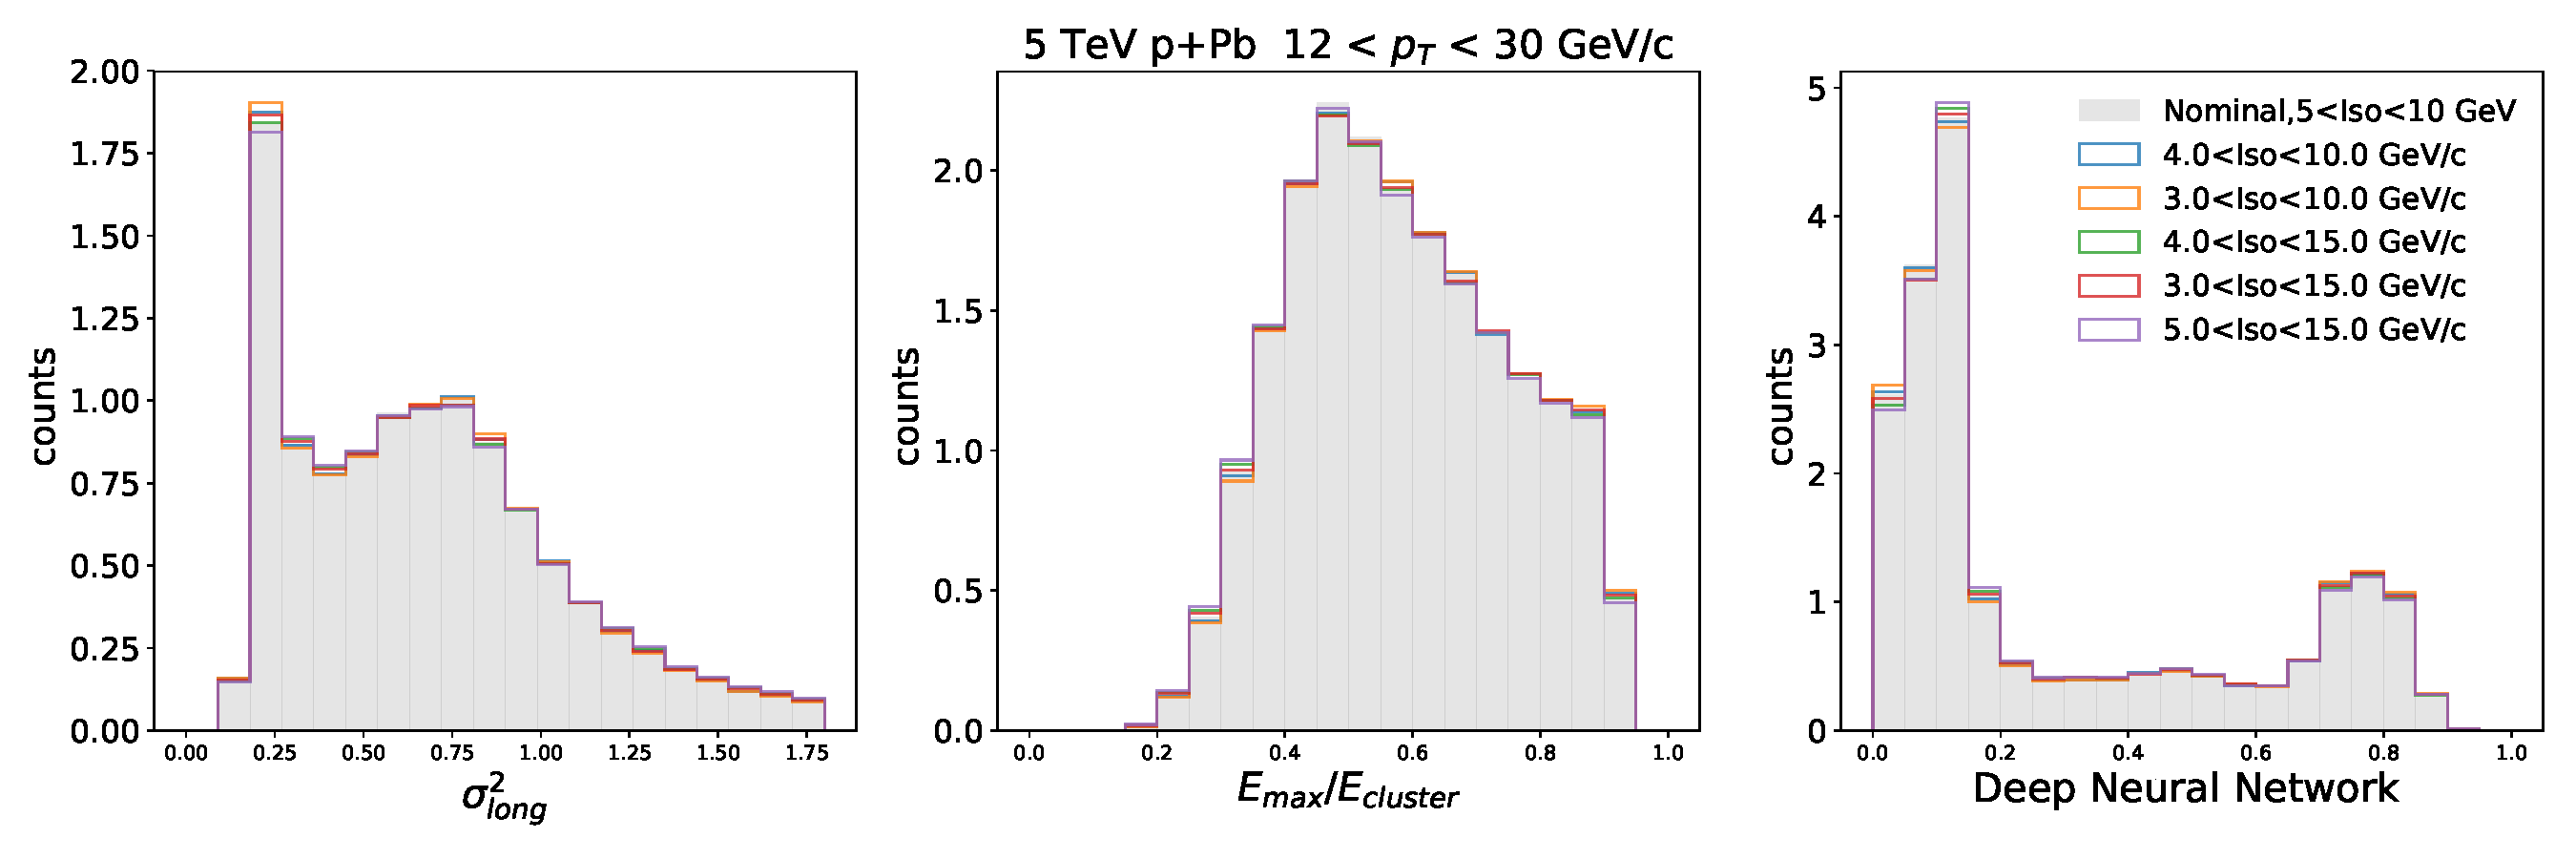
\includegraphics[width=1.0\textwidth]{Purity/IsolationCorrelationSkimmed_13def_root}\\
%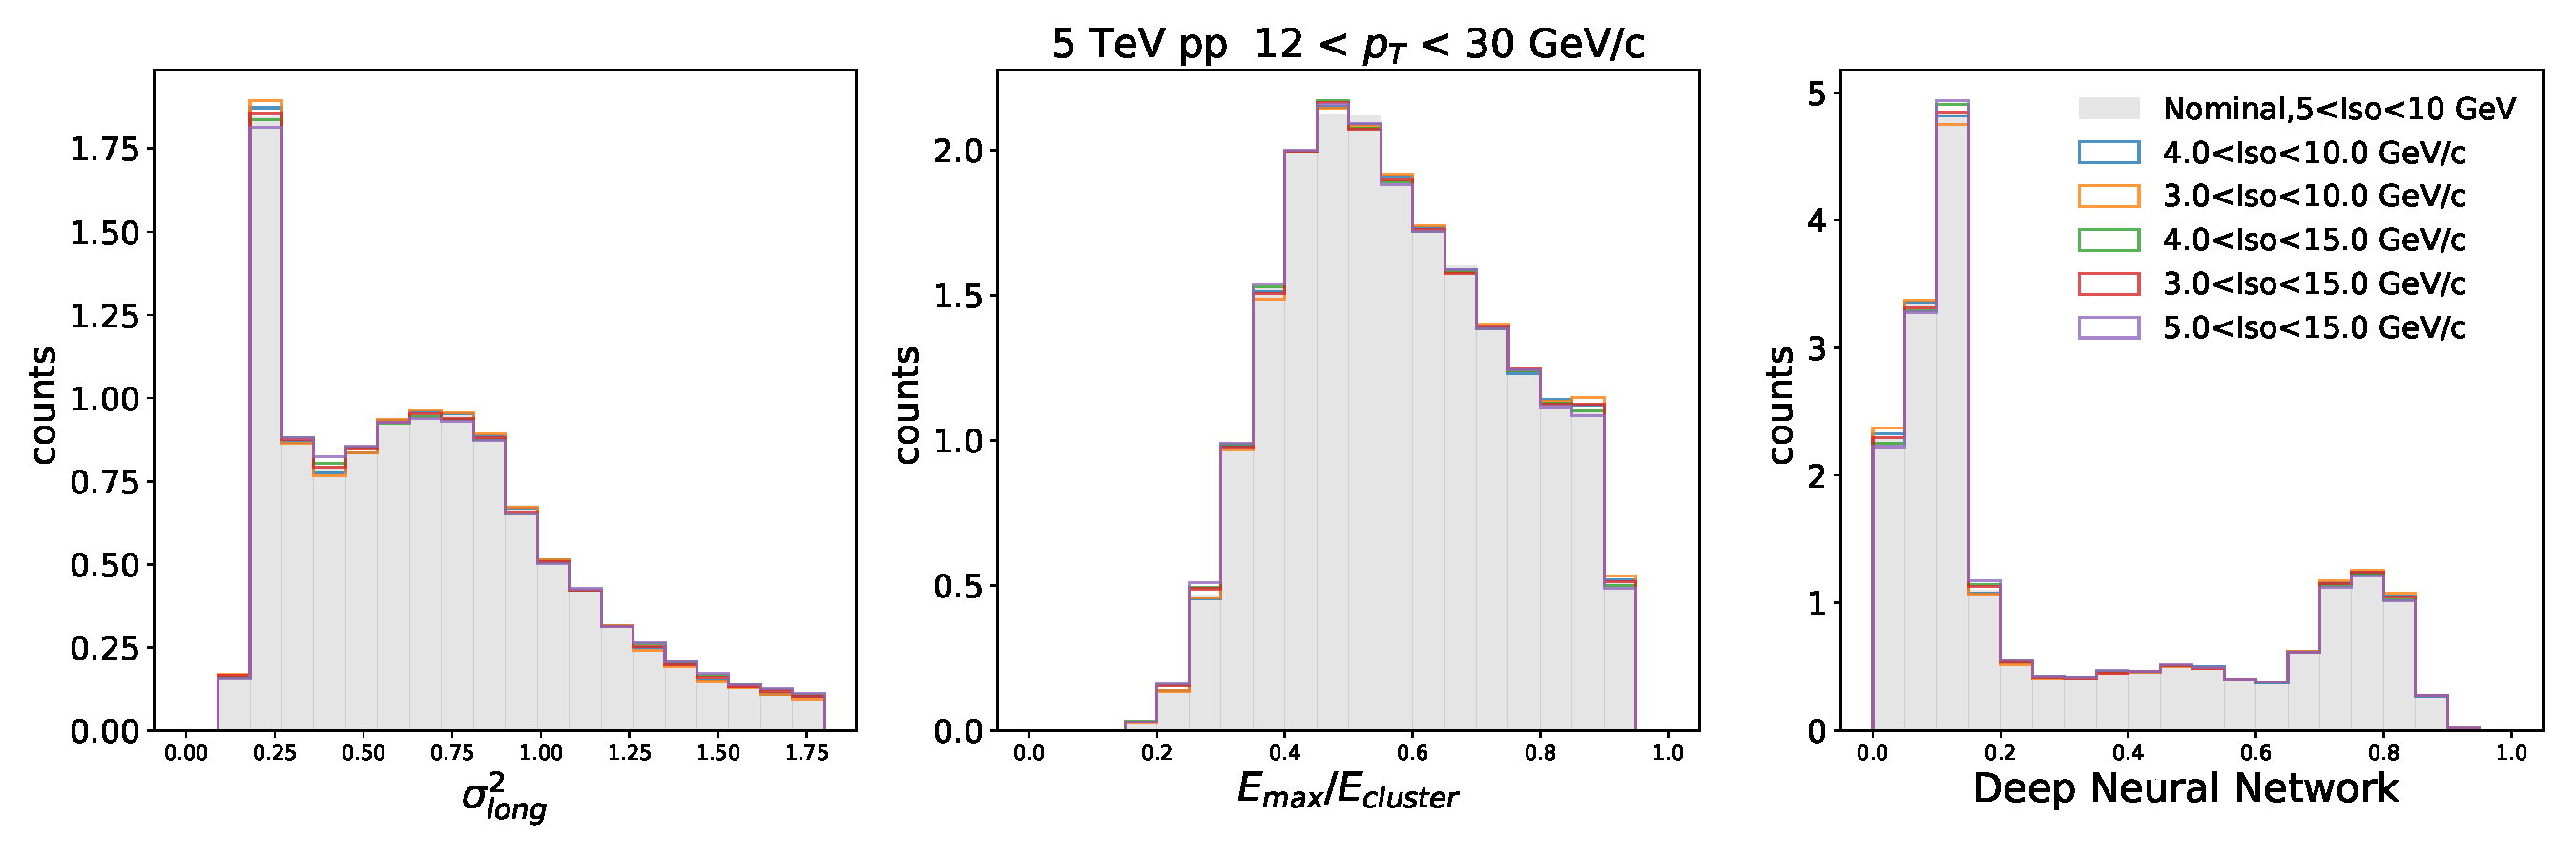
\includegraphics[width=1.0\textwidth]{Purity/IsolationCorrelationSkimmed_17q_root}
%\caption{Shower shape distributions for different anti-isolation sideband regions in pp (upper row) and p-Pb data (bottom row).}
%\label{SidebandVariation}
%\end{figure}

%Figure~\ref{SidebandVariation} shows that there is no strong dependence of the shower-shape distributions on the variations of the sideband definition, until one reaches a large value of the anti-isolation cut. This illustrates in a different way the result already shown in Figure~\ref{sidebandslices}. 

%\begin{figure}[h]
%\center
%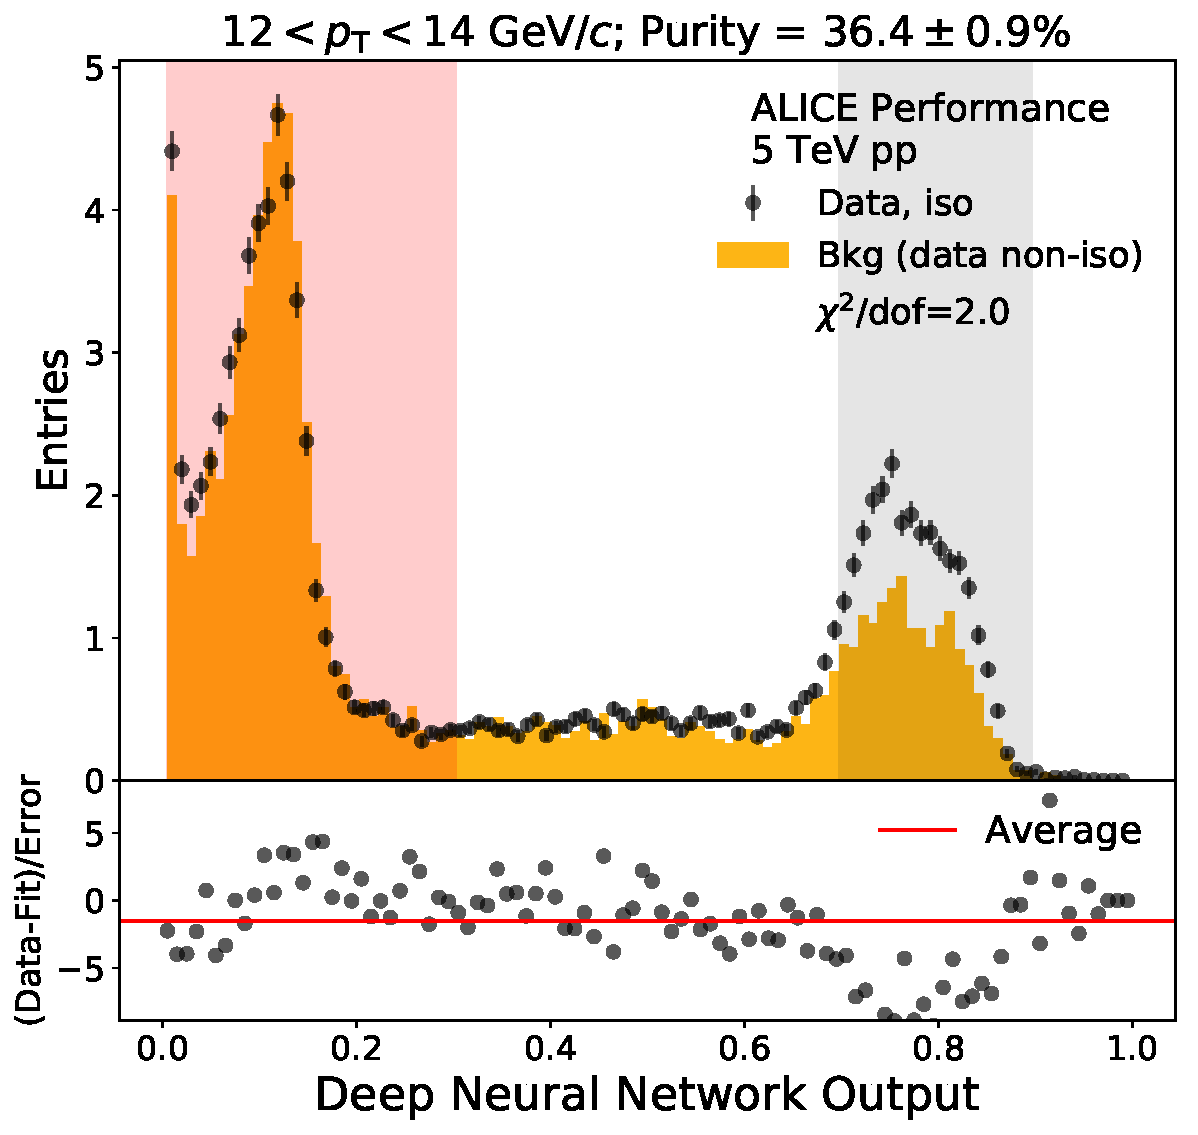
\includegraphics[width=0.49\textwidth]{Purity/bf-example-pp-cluster_NN1-12-14redbin.pdf}
%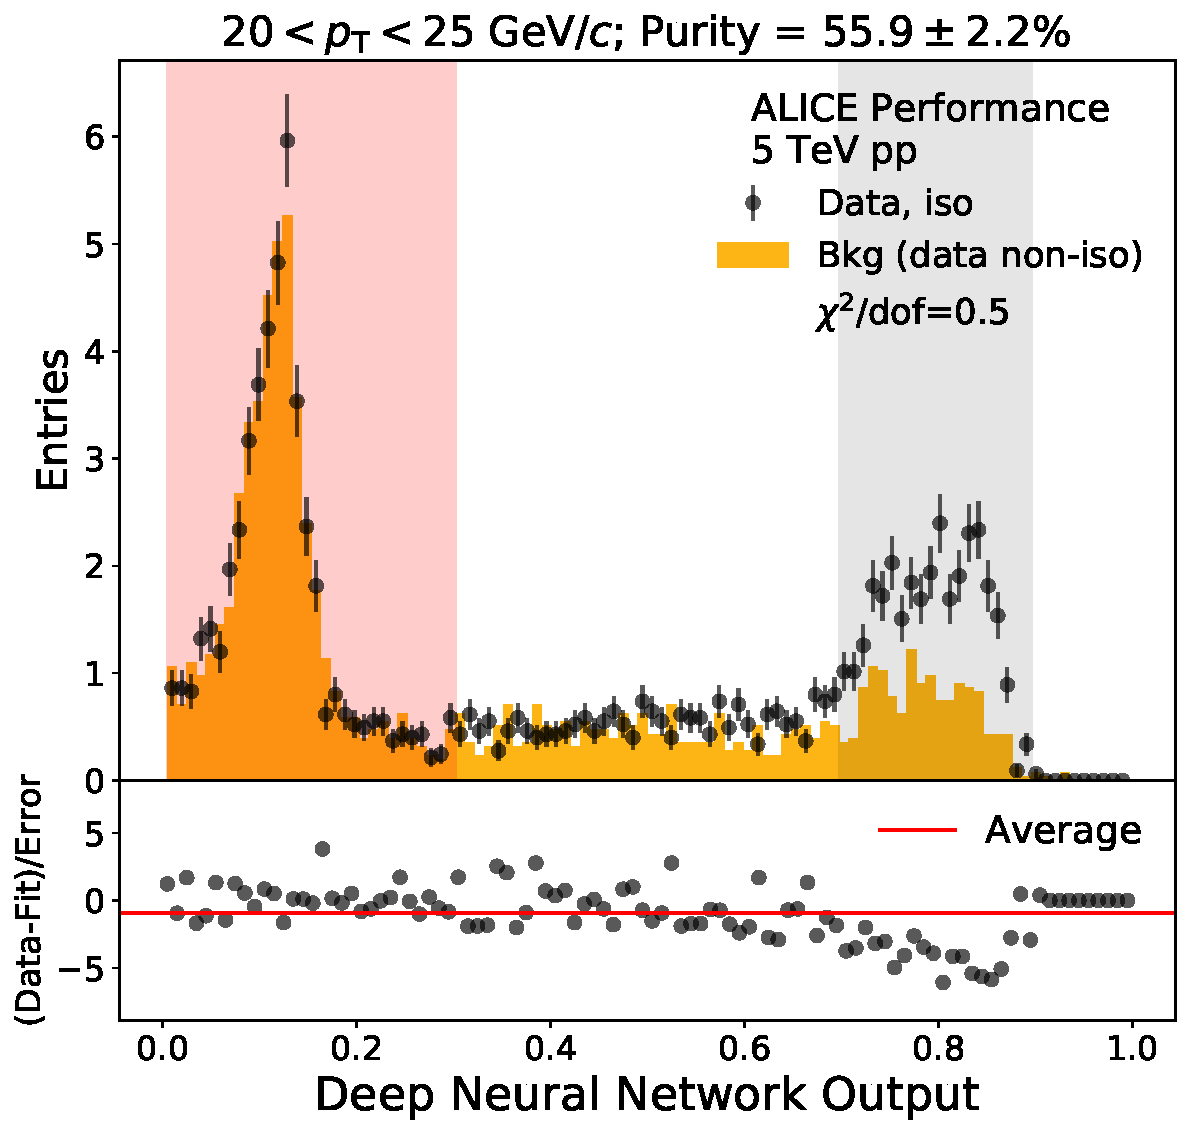
\includegraphics[width=0.49\textwidth]{Purity/bf-example-pp-cluster_NN1-20-25redbin.pdf}
%\caption{Representative fit results of background-only template method for pp data using the using the DNN and $\lambdasquare$ variables. The yellow histograms are the predicted counts given the best-fit value of the total number of clusters in the background dominated region. The hatched gray area represents the interval considered for the purity estimate. The bottom panels show the normalized residuals of the fit, considering the statistical uncertainty on the isolated data and the background template added in quadrature. }
%\label{BkgOnlyFit_pp}
%\end{figure}

%\begin{figure}[h]
%\center
%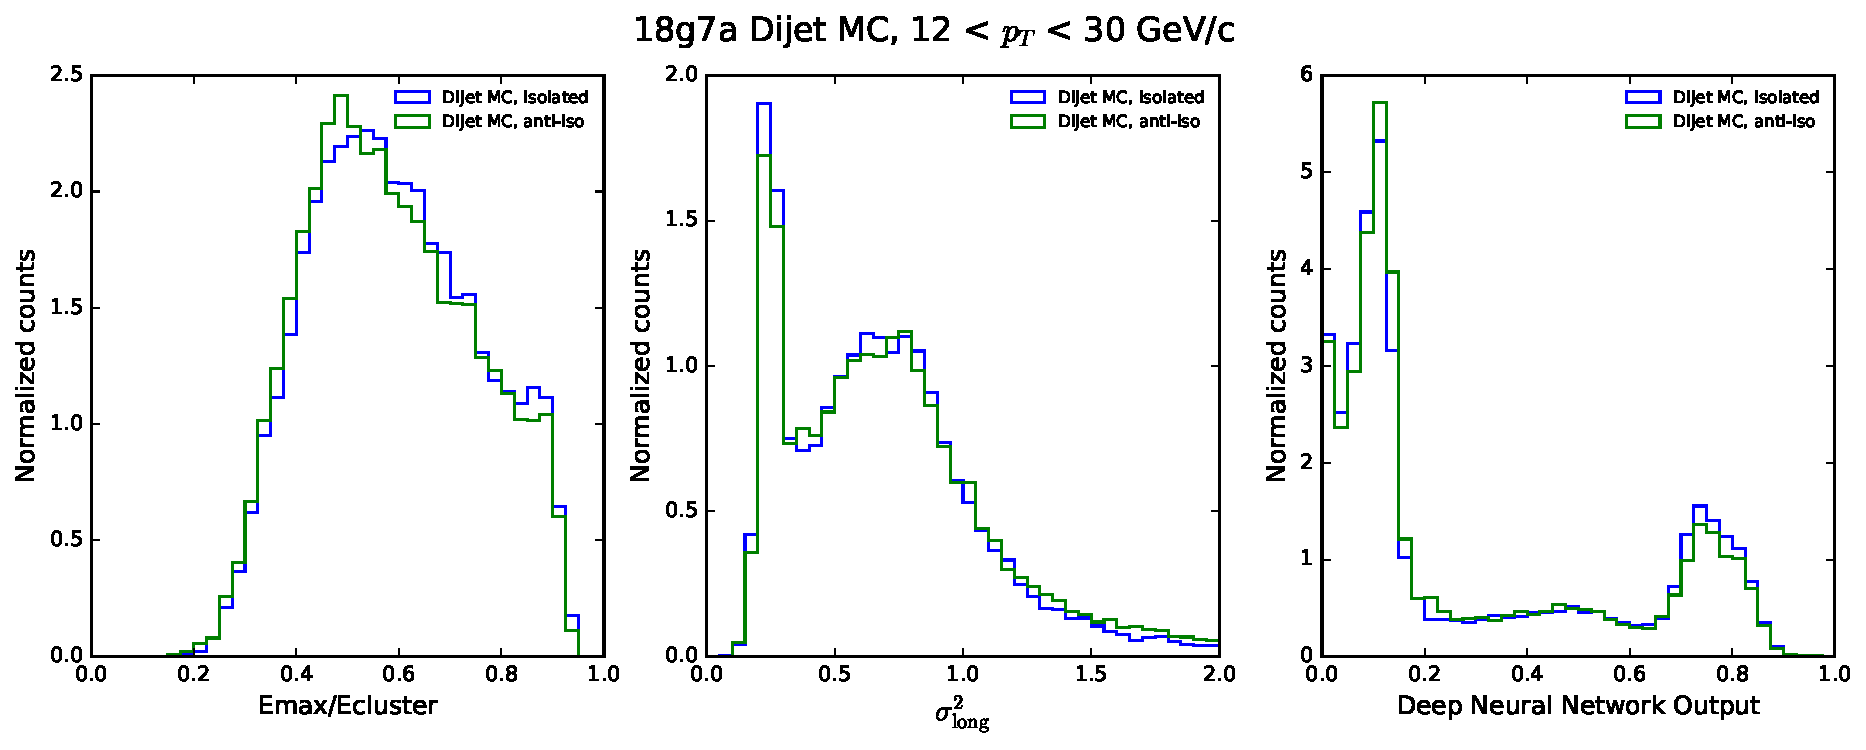
\includegraphics[width=1.0\textwidth]{Purity/bkg-template-iso-vs-antiiso.pdf}
%\caption{Background simulation of the shower-shape distributions in the signal and sideband regions for clusters with $12<\pt<30$ \GeVc.}
%\label{BKGshape}
%\end{figure}

%Figure~\ref{Erwanns} shows the purity results obtained with the ABCD method with charged only and charged + neutral energy. The results show that the purity increases, as expected, but the increase is only about $10\%$ in the range 10--16 \GeVc~and about 5$\%$ between 20--30 \GeVc. 

%\begin{figure}[h]
%\center
%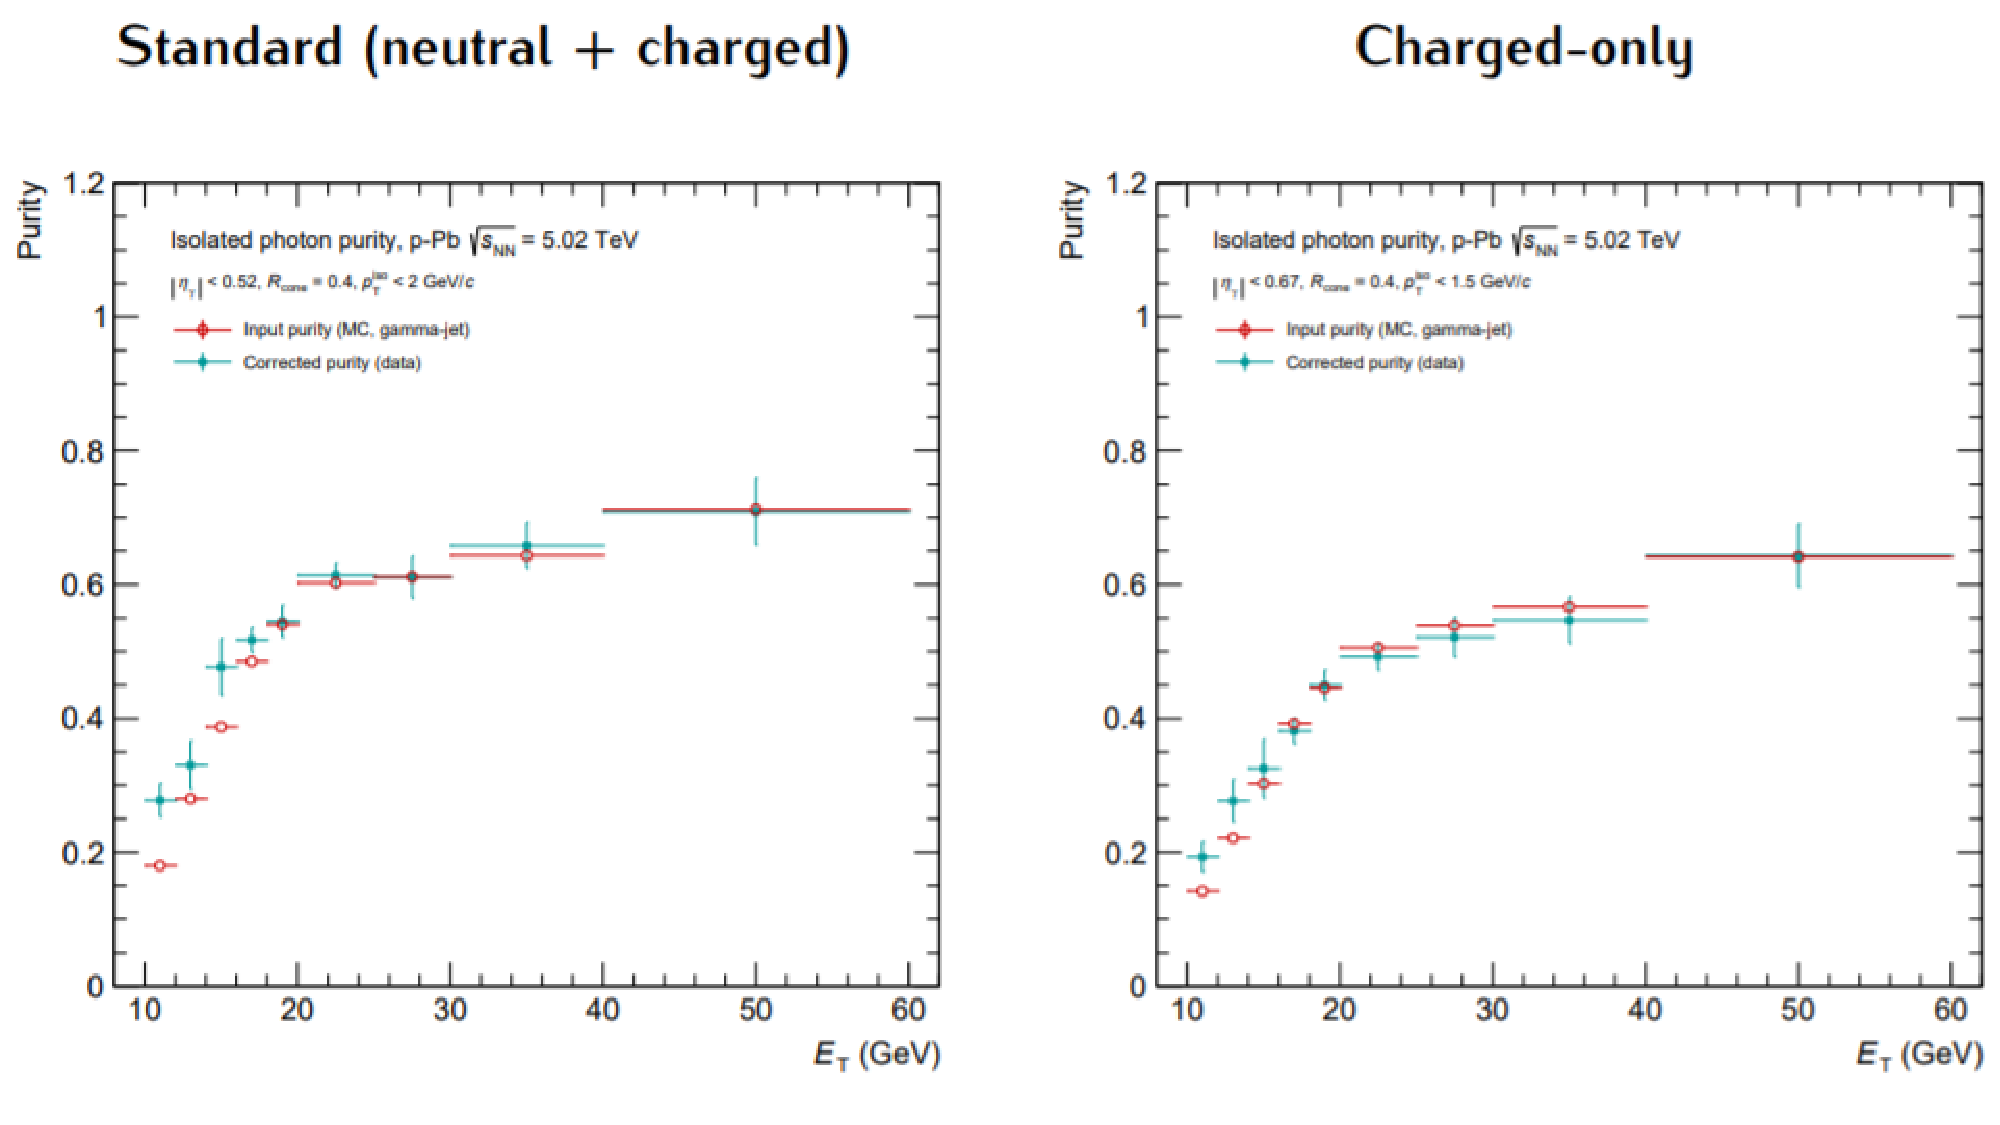
\includegraphics[width=1.0\textwidth]{Purity/ErwannsSlide}
%\caption{Purity results obtained with the ABCD method with charged+neutral (left) and charged-only (right) isolation for the 2013 p-Pb data. From slides presented by E. Masson during the Physics forum in 04/24/18. }
%\label{Erwanns}
%\end{figure}

%\subsection{Comment on neutral energy in isolation}
%\label{sec:neutraliso}
%In principle, we could expand the definition of our isolation variable to include energy measured in the calorimeters. This has been studied in the context of spectra analysis with 2013 p-Pb data~\cite{Erwann}. 

%However, the associated biases from stronger correlation between the shower-shape variable and isolation variable (needed for the purity measurements) increases for $\pi^{0}$ decays. This is visible in the results shown in the figure, especially at lower momentum, where it is less likely for a $\pi^{0}\to\gamma\gamma$ to produce a merged cluster. The correction factor is higher, as can be observed in the figure. Based on this study, we do not pursue studies on the inclusion of neutral energy in the isolation energy. A quantitative comparison of purities from the template fit and ABCD method is presented in Section~\ref{sec:comparisontoABCD}.

%This section describes the systematic uncertainty associated with our purity measurement. We estimate this independently for each shower-shape variable. As described in Section~\ref{sec:systematics}, for our final analysis we use the variables separately and estimate the uncertainty due to shower-shape definition in the final $\gammaiso$--hadron and $\gammaiso$--jet results.

%The measured purity values is compatible within a given data set and between pp and \pPb~datasets. The fact that the pp and \pPb~purities agree is not surprising given the fact that they are driven by the EMCal granularity and the $\gamma_{\mathrm{prompt}}/\pi^{0}$ cross-section ratio, which are likely very similar in both datasets. This also shows that the larger underlying event in \pPb~is appropriately subtracted; otherwise, the resulting purity would have been significantly lower due to improper UE subtraction. 

%Figure~\ref{fig:Chi2} shows the reduced $\chi^{2}$ for all the fit results presented in Table~\ref{tab:purity}. This shows than an acceptable goodness-of-fit is achieved for all the \pt~intervals considered. 

%\begin{figure}[h]
%\center
%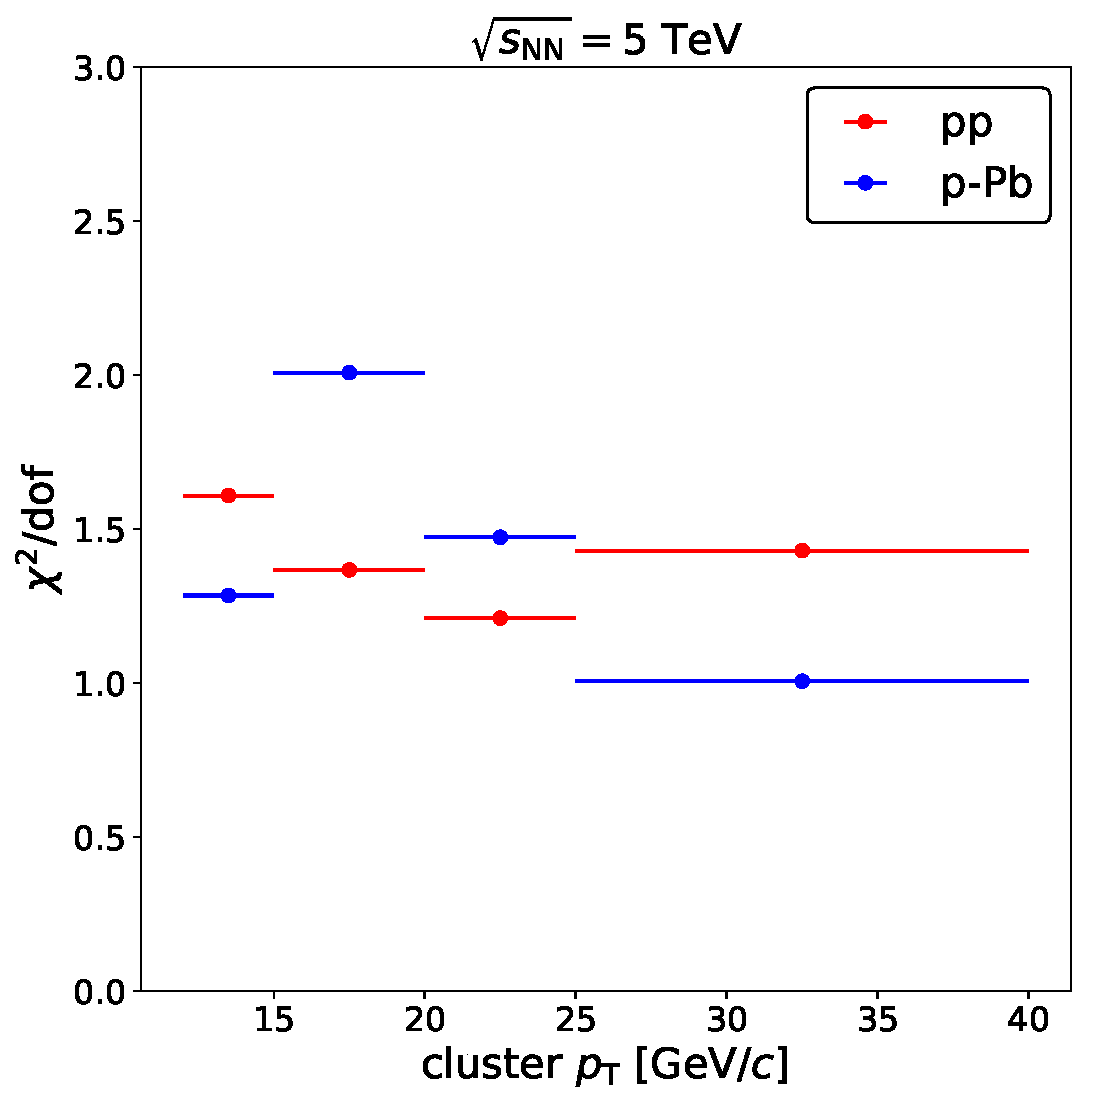
\includegraphics[width=0.495\textwidth]{Purity/combinedupdated.pdf}
%\caption{Reduced $\chi^{2}$ of template fit as a function of cluster $\pt$ for pp and \pPb~data.}
%\label{fig:Chi2}
%\end{figure}